% !TeX spellcheck = pl_PL
\documentclass[a4paper,twoside]{article}
\usepackage{polski}
\usepackage[utf8]{inputenc}
\usepackage{graphicx}
\usepackage{amsmath}

\usepackage[unicode, bookmarks=true]{hyperref} %do zakładek
\usepackage{tabto} % do tabulacji
\NumTabs{6} % globalne ustawienie wielkosci tabulacji
\usepackage{array}
\usepackage{multirow}
\usepackage{array}
\usepackage{dcolumn}
\usepackage{bigstrut}
\usepackage{color}
\usepackage[usenames,dvipsnames]{xcolor}
\usepackage{wrapfig}
\usepackage{listings,lstautogobble}


\setlength{\textheight}{24cm}
\setlength{\textwidth}{15.92cm}
\setlength{\footskip}{10mm}
\setlength{\oddsidemargin}{0mm}
\setlength{\evensidemargin}{0mm}
\setlength{\topmargin}{0mm}
\setlength{\headsep}{5mm}

\newcolumntype{M}[1]{>{\centering\arraybackslash}m{#1}}
\newcolumntype{N}{@{}m{0pt}@{}}

\graphicspath{ {./images/} }

% === Reset inkrementacji sekcji przy nowym parcie === %
\usepackage{titlesec}

\makeatletter
\@addtoreset{section}{part}
\makeatother
\titleformat{\part}[display]
{\normalfont\LARGE\bfseries\centering}{}{0pt}{}


% --- Listing dialektu SPARC Assemblera
\lstdefinelanguage
[sparc]{Assembler}		%
[x86masm]{Assembler}	% based on the "x86masm" dialect
{
	morekeywords= %
	{
		ld, LD, st, ST, %
		mov, MOV, swap, SWAP, %
		nop, NOP, %
		AND, and, ANDcc, andcc, OR, or, ORcc, orcc, XOR, xor, XORcc, xorcc, %
		ADDX, addx, ADDXcc, addxcc, %
		SUB, sub, SUBcc, subcc, SUBX, subx, SUBXcc, subxcc, %
		UMUL, umul, SMUL, smul, UMULcc, umulcc, SMULcc, smulcc, %
		UDIV, udiv, SDIV, sdiv, UDIVcc, udivcc, SDIVcc, sdivcc, %
		BA, ba, BNE, bne, BG, bg, BNEG, bneg%
		CALL, call, RET, ret, RETL, retl, %
		SAVE, save, RESTORE, restore %
	}	
}

% --- Opcje listingu kodu
\lstset{
	frame=single,
	autogobble=true,
	commentstyle=\ttfamily\itshape\color{gray},
	keywordstyle=\color{blue},
	frameround=ffff,
	rulecolor=\color{black},
	tabsize=4,
	breaklines=true, %
	% --- Polskie znaki w listingu kodu
	literate=%
	{ą}{{\c{a}}}1
	{ć}{{\'c}}1
	{ę}{{\c{e}}}1
	{ł}{{\l{}}}1
	{ń}{{\'n}}1
	{ó}{{\'o}}1
	{ś}{{\'s}}1
	{ź}{{\'z}}1
	{ż}{{\.z}}1
	{Ą}{{\c{A}}}1
	{Ć}{{\'C}}1
	{Ę}{{\c{E}}}1
	{Ł}{{\L{}}}1
	{Ń}{{\'N}}1
	{Ó}{{\'O}}1
	{Ś}{{\'S}}1
	{Ź}{{\'Z}}1
	{Ż}{{\.Z}}1
}

\begin{document}
\bibliographystyle{plain}
% === DEFINICJA ZIELONEGO ==================== %
\definecolor{Gurin}{rgb}{0, 0.35, 0}

% === MAKRODEFINICJA POPRAWNEJ I ZŁEJ ODPOWIEDZI ==================== %
\newcommand{\Tak}[1] {
	\color{Gurin}{#1}
}
\newcommand{\Nie}[1] {
	\color{Red}{#1}
}

% === Porównywarka odpowiedzi
\newcommand{\answer}[3] {
	\ifnum\pdfstrcmp{#1}{Tak}=0
	\Tak{\item \textbf{#2}}
	\else
	\Nie{\item #2}
	\fi
	\if\relax\detokenize{#3}\relax
	\else
	\\
	\fi
	\color{Black}{\emph{#3}}\\
}

% === MAKRODEFINICJA PYTANIA I ODPOWIEDZI =========================== %
\newcommand{\question}[2]{ %
	\setkeys{Question}{#1} %
	\begin{itemize}
		\setkeys{Answers}{#2}
	\end{itemize}
}

% definicje treści pytania i odpowiedzi
\makeatletter
\define@key{Question}{question}{\item \textbf{#1}}
\define@key{Answers}{isTrue1}{\def\QA@isTrueI{#1}}
\define@key{Answers}{answer1}{\def\QA@answerI{#1}}
\define@key{Answers}{explain1}{\answer{\QA@isTrueI}{\QA@answerI}{#1}}
\define@key{Answers}{isTrue2}{\def\QA@isTrueII{#1}}
\define@key{Answers}{answer2}{\def\QA@answerII{#1}}
\define@key{Answers}{explain2}{\answer{\QA@isTrueII}{\QA@answerII}{#1}}
\define@key{Answers}{isTrue3}{\def\QA@isTrueIII{#1}}
\define@key{Answers}{answer3}{\def\QA@answerIII{#1}}
\define@key{Answers}{explain3}{\answer{\QA@isTrueIII}{\QA@answerIII}{#1}}
\define@key{Answers}{isTrue4}{\def\QA@isTrueIV{#1}}
\define@key{Answers}{answer4}{\def\QA@answerIV{#1}}
\define@key{Answers}{explain4}{\answer{\QA@isTrueIV}{\QA@answerIV}{#1}}
\define@key{Answers}{isTrue5}{\def\QA@isTrueV{#1}}
\define@key{Answers}{answer5}{\def\QA@answerV{#1}}
\define@key{Answers}{explain5}{\answer{\QA@isTrueV}{\QA@answerV}{#1}}
\define@key{Answers}{isTrue6}{\def\QA@isTrueVI{#1}}
\define@key{Answers}{answer6}{\def\QA@answerVI{#1}}
\define@key{Answers}{explain6}{\answer{\QA@isTrueVI}{\QA@answerVI}{#1}}
\define@key{Answers}{isTrue7}{\def\QA@isTrueVII{#1}}
\define@key{Answers}{answer7}{\def\QA@answerVII{#1}}
\define@key{Answers}{explain7}{\answer{\QA@isTrueVII}{\QA@answerVII}{#1}}
\define@key{Answers}{isTrue8}{\def\QA@isTrueVIII{#1}}
\define@key{Answers}{answer8}{\def\QA@answerVIII{#1}}
\define@key{Answers}{explain8}{\answer{\QA@isTrueVIII}{\QA@answerVIII}{#1}}
\define@key{Answers}{isTrue9}{\def\QA@isTrueIX{#1}}
\define@key{Answers}{answer9}{\def\QA@answerIX{#1}}
\define@key{Answers}{explain9}{\answer{\QA@isTrueIX}{\QA@answerIX}{#1}}
\define@key{Answers}{isTrue10}{\def\QA@isTrueX{#1}}
\define@key{Answers}{answer10}{\def\QA@answerX{#1}}
\define@key{Answers}{explain10}{\answer{\QA@isTrueX}{\QA@answerX}{#1}}




\begin{titlepage}
\title{\huge Architektura komputerów - ULTIMATE}
\author{\large SonMati \\ Doxus}
\maketitle
\end{titlepage}

% !TeX spellcheck = pl_PL

\newpage
%===============================================================================
%*** Opracowanie wykładów *****************************
%===============================================================================
\part{Teoria}


%========================================
%*** Historia rozwoju komputerów ********
%========================================
\section{Historia rozwoju komputerów}
	\begin{enumerate}
	    \item Liczydło
	    \item Pascalina - maszyna licząca Pascala (dodawanie i odejmowanie)
	    \item Maszyna mnożąca Leibniza (dodawanie, odejmowanie, mnożenie, dzielenie, pierwiastek kwadratowy
	    \item Maszyna różnicowa - Charles Babbage, obliczanie wartości matematycznych do tablic
	    \item Maszyna analityczna - Charles Babvage, programowalna za pomocą kart perforowanych
	  	\item Elektryczna maszyna sortująca i tabelaryzująca Holleritha 1890
	    \item Kalkulator elektromechaniczny Mark I, tablicowanie funkcji, całkowanie numeryczne, rozwiązywanie równań różniczkowych, rozwiązywanie układów równań liniowych, analiza harmoniczna, obliczenia statystyczne
	    \item Maszyny liczące Z1: pamięć mechaniczna, zmiennoprzecinkowa reprezentacja liczb, binarna jednostka zmiennoprzecinkowa
	    \item Z3: Pierwsza maszyna w pełni automatyczna, kompletna w sensie Turinga, pamięć przekaźnikowa
	    \item Colossus i Colossus 2
	    \item ENIAC
	    \item EDVAC - J. von Neumann (wtedy utworzył swoją architekturę) \\
	    	\begin{figure}[h]
			\centering
			%\includegraphics[scale=0.1]{architektura_von_Neumanna.png}
			\end{figure}
	    \item UNIVAC I (pierwszy udany komputer komercyjny)
	    \item IBM 701, potem 709
	    \item po 1955 zaczyna się zastosowanie tranzystorów w komputerach (komputery II generacji)
	    \item po 1965 komputery III generacji z układami scalonymi
	    \item od 1971 komputery IV generacji - z układami scalonymi wielkiej skali inegracji VLSI
    \end{enumerate}
    

%========================================
%*** Architektura CISC ******************
%========================================
\section{Architektura CISC}
	\subsection{Znaczenie} \noindent
		Complex Instruction Set Computers
	
	\subsection{Przyczyny rozwoju architektury CISC}
    	\begin{itemize}
	        \item Drogie, małe i wolne pamięci komputerów
	        \item Rozwój wielu rodzin komputerów
	        \item Duża popularność mikroprogramowalnych układów sterujących (prostych w rozbudowie)
	        \item Dążenie do uproszczenia kompilatorów. Im więcej będzie rozkazów maszynowych odpowiadających instrukcjom języków wyższego poziomu tym lepiej.
        \end{itemize}
    
    \subsection{Cechy architektury CISC}
    	\begin{itemize}
	        \item Duża liczba rozkazów (z czego te najbardziej zaawansowane i tak nie były używane)
	        \item Duża ilość trybów adresowania (związane z modelem obliczeń)
	        \item Duży rozrzut cech rozkazów w zakresie:
	        \begin{itemize}
		        \item złożoności
		        \item długości (szczególnie to - nawet kilkanaście bajtów)
		        \item czasów wykonania
	        \end{itemize}
	        \item Model obliczeń pamięć - pamięć
	        \item Niewiele rejestrów - były droższe niż komórki pamięci i przy przełączaniu kontekstu obawiano się wzrostu czasu przełączania kontekstu (chowanie rejestrów na stos i odwrotnie)
        \end{itemize}
   
   \textbf{\large CIEKAWOSTKA:} Przeanalizowano jakieś tam programy i w procesorze VAX 20\% najbardziej złożonych rozkazów odpowiadało za 60\% kodu, stanowiąc przy tym ok 0.2\% wywołań.\\ W procesorze MC68020 71\% rozkazów nie zostało nawet użytych w badanych programach
   
	\section{Architektura RISC}
		\subsection{Znaczenie} \noindent
			Reduced Instruction Set Computers
   		\subsection*{Przyczyny rozwoju}
	   		\begin{itemize}
	   			\item Poszukiwanie optymalnej listy rozkazów
	   			\item Chęć wykonania mikroprocesora o funkcjach pełnego ówczesnego procesora
	   		\end{itemize}
   		
   		\subsection{Pierwszy procesor RISC} \noindent
	   		Procesor RISC I (1980), D. Patterson (Berkeley University)\\
	   		Założenia projektowe:
	   		\begin{itemize}
	   			\item Wykonanie jednego rozkazu w jednym cyklu maszynowym
	   			\item Stały rozmiar rozkazów – uproszczenie metod adresacji
	   			\item Model obliczeń rejestr – rejestr: komunikacja z pamięcią operacyjną tylko za pomocą rozkazów LOAD i STORE.
	   			\item Wsparcie poprzez architekturę języków wysokiego poziomu.
	   		\end{itemize}
	   		Efekty realizacji fizycznej:
	   		\begin{itemize}
	   			\item 44 420 tranzystorów (ówczesne procesory CISC zawierały ok. 100 000 tranzystorów)
	   			\item lista rozkazów = 32 rozkazy
	   			\item dwustopniowy potok – strata tylko 6\% cykli zegara, zamiast 20\% (w związku z realizacją skoków)
	   		\end{itemize}
   		
   		\subsection{Cechy architektury RISC}
	   		\begin{enumerate}
	   			\item Stała długość i prosty rozkaz formatu
	   			\item Nieduża liczba trybów adresowania
	   			\item Niezbyt obszerna lista rozkazów
	   			\item Model obliczeń rejestr-rejestr - dostęp do pamięci operacyjnej tylko w rozkazach LOAD i STORE
	   			\item Duży zbiór rejestrów uniwersalnych
	   			\item Układ sterowania – logika szyta
	   			\item Intensywne wykorzystanie przetwarzania potokowego
	   			\item Kompilatory o dużych możliwościach optymalizacji potoku rozkazów
	   		\end{enumerate}
   		
   		\subsection{Format rozkazu procesora RISC I}
	   		\begin{table}[h]
	   			\begin{tabular}{clclll}
	   				\hline
	   				\multicolumn{1}{|c|}{7}      & \multicolumn{1}{c|}{1}   & \multicolumn{1}{c|}{5}    & \multicolumn{1}{c|}{5}    & \multicolumn{1}{c|}{1}   & \multicolumn{1}{c|}{13}   \\ \hline
	   				\multicolumn{1}{|c|}{OPCODE} & \multicolumn{1}{c|}{SCC} & \multicolumn{1}{c|}{DEST} & \multicolumn{1}{c|}{SRC1} & \multicolumn{1}{c|}{IMM} & \multicolumn{1}{c|}{SRC2} \\ \hline
	   			\end{tabular}
	   		\end{table}
	   		\begin{itemize}
	   			\item OPCODE–kod rozkazu
	   			\item SCC – ustawianie (lub nie) kodów warunków
	   			\item DEST – nr rejestru wynikowego
	   			\item SRC1 – nr rejestru zawierającego pierwszy argument
	   			\item IMM – wskaźnik natychmiastowego trybu adresowania
	   			\item SRC2 – drugi argument lub nr rejestru (na 5 bitach)
	   		\end{itemize}
   		
   		\subsection{Realizacja wybranych rozkazów}
   			\subsubsection{Rozkazy arytmetyczne}
	   			\begin{itemize}
	   				\item \textbf{Tryb rejestrowy}:\tab(IMM=0) \tab R[DEST] $\leftarrow$ R[SRC1] op R[SRC2]
	   				\item \textbf{Tryb natychmiastowy:}\tab(IMM=1) \tab{R[DEST] $\leftarrow$ R[SRC1] op SRC2}
	  			\end{itemize}
        	\subsubsection{Rozkazy komunikujące się z pamięcią}
	        	\begin{itemize}
	        		\item \textbf{LOAD}\tab{R[DEST] $\leftarrow$ M[AE]P}
	        		\item \textbf{STORE}\tab{M[AE]  $\leftarrow$ R[DEST]}
	        	\end{itemize}
        	\subsubsection{Adres efektywny}
	        	\begin{itemize}
	        		\item \textbf{Tryb z przesunięciem}\tab\tab AE = R[SRC1] + SRC2 = RX + S2
	        		\item \textbf{Inny zapis powyższego}\tab\tab AE = RX + S2
	        		\item \textbf{Tryb absolutny}\tab\tab AE = R0 + S2 = S2 (R0 $\equiv$ 0)
	        		\item \textbf{Tryb rejestrowy pośredni}\tab AE = RX + 0 = RX
	        	\end{itemize}
	        	Tryb absolutny oraz tryb rejestrowy pośredni są przypadkami szczególnymi.

	\newpage
    \subsection{Logiczna organizacja rejestrów procesora RISC I}
	    \begin{table}[htbp]
	    	\centering
	    	\caption{Rejestry}
	    	\begin{tabular}{c|c|c}
	    		\cline{2-2}    \multirow{4}[2]{*}{6} & \multirow{4}[2]{*}{Wysokie} & {\scriptsize R31} \bigstrut[t]\\
	    		&       &  \\
	    		&       &  \\
	    		&       &  \bigstrut[b]\\
	    		\cline{2-2}    \multirow{4}[2]{*}{10} & \multirow{4}[2]{*}{Lokalne} &  \bigstrut[t]\\
	    		&       &  \\
	    		&       &  \\
	    		&       &  \bigstrut[b]\\
	    		\cline{2-2}    \multirow{4}[2]{*}{6} & \multirow{4}[2]{*}{Niskie} &  \bigstrut[t]\\
	    		&       &  \\
	    		&       &  \\
	    		&       &  \bigstrut[b]\\
	    		\cline{2-2}    \multirow{4}[2]{*}{10} & \multirow{4}[2]{*}{Globalne} & {\scriptsize R9} \bigstrut[t]\\
	    		&       &  \\
	    		&       &  \\
	    		&       & {\scriptsize R0} \bigstrut[b]\\
	    		\cline{2-2}    \end{tabular}%
	    	\label{tab:addlabel}%
	    	\vspace{-2cm}
	    \end{table}
	\subsection{Okno rejestrów}
	    \begin{table}[htbp]
	    	\centering
	    	\caption{Rejestry fizyczne}
	    	\begin{tabular}{r|r|r}
	    		\cline{2-2}    137   & \multirow{6}[2]{*}{$ \uparrow $ Okno rejestrów} &  \bigstrut[t]\\
	    		&       &  \\
	    		&       &  \\
	    		&       &  \bigstrut[b]\\
	    		\cline{2-2}          & \multicolumn{1}{c|}{\multirow{4}[2]{*}{Wysokie}} & \multicolumn{1}{c}{R31} \bigstrut[t]\\
	    		& \multicolumn{1}{c|}{} & \multicolumn{1}{c}{} \\
	    		& \multicolumn{1}{c|}{} & \multicolumn{1}{c}{} \\
	    		& \multicolumn{1}{c|}{} & \multicolumn{1}{c}{} \bigstrut[b]\\
	    		\cline{2-2}          & \multicolumn{1}{c|}{\multirow{4}[2]{*}{Lokalne}} & \multicolumn{1}{c}{} \bigstrut[t]\\
	    		& \multicolumn{1}{c|}{} & \multicolumn{1}{c}{} \\
	    		& \multicolumn{1}{c|}{} & \multicolumn{1}{c}{} \\
	    		& \multicolumn{1}{c|}{} & \multicolumn{1}{c}{} \bigstrut[b]\\
	    		\cline{2-2}          & \multicolumn{1}{c|}{\multirow{4}[2]{*}{Niskie}} & \multicolumn{1}{c}{} \bigstrut[t]\\
	    		& \multicolumn{1}{c|}{} & \multicolumn{1}{c}{} \\
	    		& \multicolumn{1}{c|}{} & \multicolumn{1}{c}{} \\
	    		& \multicolumn{1}{c|}{} & \multicolumn{1}{c}{} \bigstrut[b]\\
	    		\cline{2-2}          & \multicolumn{1}{c|}{\multirow{4}[2]{*}{Globalne}} & \multicolumn{1}{c}{} \bigstrut[t]\\
	    		& \multicolumn{1}{c|}{} & \multicolumn{1}{c}{} \\
	    		& \multicolumn{1}{c|}{} & \multicolumn{1}{c}{} \\
	    		& \multicolumn{1}{c|}{} & \multicolumn{1}{c}{R0} \bigstrut[b]\\
	    		\cline{2-2}          & \multicolumn{1}{c|}{\multirow{2}[2]{*}{$ \downarrow $ }} &  \bigstrut[t]\\
	    		& \multicolumn{1}{c|}{} &  \\
	    		0     & \multicolumn{1}{c|}{} &  \bigstrut[b]\\
	    		\cline{2-2}
	    	\end{tabular}%
	    	\label{tab:addlabel}%
	    \end{table}
	    
	    % --- OBRAZKI
%	    \begin{center}
%	    	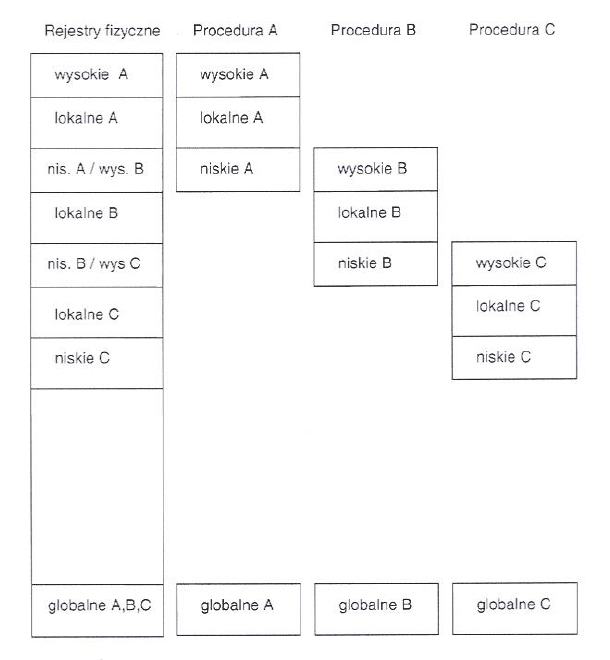
\includegraphics[width=10cm]{RISC_proc1}
%	    \end{center}
%	    \begin{center}
%	    	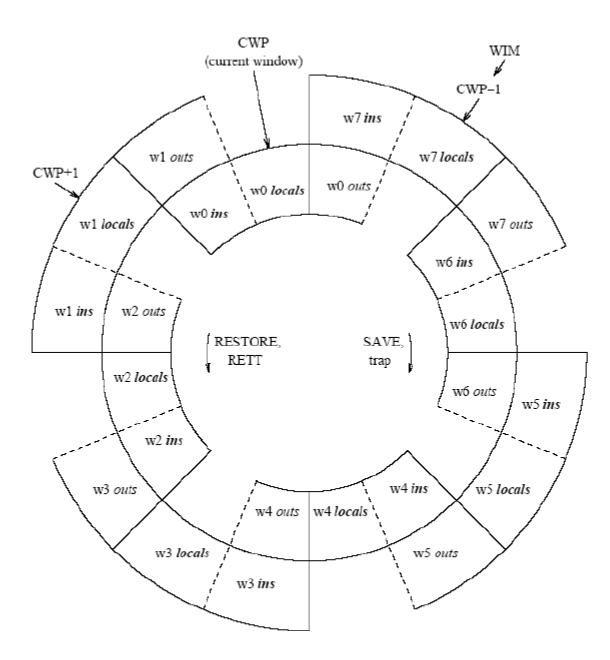
\includegraphics[width=10cm]{RISC_proc2}
%	    \end{center}
	    
	\pagebreak
\section{Mechanizmy potokowe}
	\subsection{Realizacja rozkazów w procesorze niepotokowym}
		Rozkazy wykonywane są liniowo w czasie - jeden po drugim, w takiej kolejności w jakiej przyjdą do procesora.
   	\subsection{Potokowe wykonanie rozkazówdla prostej organizacji cyklu rozkazowego}
   		Prosty podział procesora na moduły:
	   	\begin{itemize}
	   		\item S1 - pobranie rozkazu
	   		\item S2 - wykonanie rozkazu
	   	\end{itemize}
   		Zakładając, że czas pracy obu modułów jest równy, wówczas 3 rozkazy mogą zostać wykonane w 2 okresach.\\
   		1 T - pobranie i wykonanie rozkazu. W momencie gdy pierwszy rozkaz zostanie pobrany, w chwili 0.5 T S1 może pobrać kolejny.
   	\subsection{Podział cyklu rozkazowego na większą liczbę faz}
   		Na przykładzie cyklu rozkazowego komputera Amdahl 470
	   	\begin{enumerate}
	   		\item Pobranie rozkazu
	   		\item Dekodowanie rozkazu
	   		\item Obliczenie adresu efektywnego
	   		\item Pobranie argumentów
	   		\item Wykonanie operacji
	   		\item Zapis wyniku
	   	\end{enumerate}
	   	Zasada działania jest dokładnie taka sama jak w przypadku podziału na dwie fazy. Załóżmy, że jeden rozkaz wykonuje się w 7iu taktach zegarowych. 1 T = 7 F. Wówczas w momencie gdy rozkaz numer 1 znajduje się w 5tym takcie wykonania rozkaz numer 5 może zostać pobrany.
   
	   	\begin{table}[htbp]
	   		\centering
	   		\caption{Zobrazowanie potoku}
	   		\begin{tabular}{|r|r|r|r|r|r|r|r|r|}
	   			\multicolumn{1}{r}{Rozkazy} & \multicolumn{1}{r}{} & \multicolumn{7}{c}{Fazy zegarowe} \\
	   			\multicolumn{1}{r}{} & \multicolumn{1}{r}{} & \multicolumn{1}{c}{1} & \multicolumn{1}{c}{2} & \multicolumn{1}{c}{3} & \multicolumn{1}{c}{4} & \multicolumn{1}{c}{5} & \multicolumn{1}{c}{6} & \multicolumn{1}{c}{7} \bigstrut[b]\\
	   			\cline{1-1}\cline{3-9}    \multicolumn{1}{|c|}{S1} &       & r1    & r2    & r3    & r4    & r5    & r6    & r7 \bigstrut\\
	   			\cline{1-1}\cline{3-9}    \multicolumn{1}{|c|}{S2} &       &       & r1    & r2    & r3    & r4    & r5    & r6 \bigstrut\\
	   			\cline{1-1}\cline{3-9}    \multicolumn{1}{|c|}{S3} &       &       &       & r1    & r2    & r3    & r4    & r5 \bigstrut\\
	   			\cline{1-1}\cline{3-9}    \multicolumn{1}{|c|}{S4} &       &       &       &       & r1    & r2    & r3    & r4 \bigstrut\\
	   			\cline{1-1}\cline{3-9}    \multicolumn{1}{|c|}{S5} &       &       &       &       &       & r1    & r2    & r3 \bigstrut\\
	   			\cline{1-1}\cline{3-9}    \multicolumn{1}{|c|}{S6} &       &       &       &       &       &       & r1    & r2 \bigstrut\\
	   			\cline{1-1}\cline{3-9}    \end{tabular}%
	   		\label{tab:addlabel}%
	   	\end{table}%
	   
   	\subsection{Analiza czasowa potokowej realizacji ciągu rozkazów}
   		Założenia
	   	\begin{itemize}
	   		\item \textbf{P} - liczba faz
	   		\item \textbf{T} - okres
	   		\item $\frac{T}{P}=\tau $ - czas wykonania pojedynczej fazy
	   	\end{itemize}
   		$(n-1)\times\tau$ - czas rozpoczęcia wykonywania \emph{n}-tego rozkazu.
   	\subsection{Czas wykonywania rozkazów}
	   	\begin{itemize}
	   		\item W procesorze niepotokowym\\
	   		$t=n\times T$ - dla \emph{n} rozkazów
	   		\item W procesorze potokowym dla idealnego przypadku, gdy $\tau=\frac{T}{P}$\\
	   		$t=(n-1)\times\tau+T=(n-1+P)\times\frac{T}{P}$
	   	\end{itemize}
   	\subsection{Przyspieszenie dla potokowego wykonania rozkazów}
	   	Przyspieszenie jest stosunkiem czasu wykonywania rozkazów dla procesora niepotokowego do czasu dla procesora potokowego.\\\\
	   	$\lim_{n \to \infty}\frac{n\times T}{(n-1+P)\times\frac{T}{P}}=P$\\\\
	   	Maksymalne przyspieszenie (dla modelu idealnego) jest równe ilości faz.
   	\subsection{Problemy z potokową realizacją rozkazów}
   		Problemem związanym z realizacją potokową jest \textbf{zjawisko hazardu}.
	   	\begin{itemize}
	   		\item \textbf{Hazard sterowania }– problemy z potokową realizacją skoków i rozgałęzień.
	   		\item \textbf{Hazard danych} – zależności między argumentami kolejnych rozkazów
	   		\item \textbf{Hazard zasobów} – konflikt w dostępie do rejestrów lub do pamięci
	   	\end{itemize}
   	\subsection{Rozwiązanie problemu hazardu sterowania}
	   	\begin{itemize}
	   		\item Skoki opóźnione
	   		\item Przewidywanie rozgałęzień
	   	\end{itemize}
   	\subsection{Skoki opóźnione}
	   	\subsubsection{Założenia}
		   	\begin{itemize}
		   		\item Rozkaz następny po skoku jest zawsze całkowicie wykonywany
		   		\item To znaczy, że efekt skoku jest opóźniony o jeden rozkaz
		   	\end{itemize}
   		\subsubsection{Działanie}
   			Zmienia kod programu w trakcie kompilacji, jeśli widzi taka potrzebę. Sprowadza się to do dwóch możliwości:
		   	\begin{itemize}
		   		\item Modyfikacja programu - dodanie rozkazu NOP po instrukcji skoku JMP
		   		\item Optymalizacja programu - zmiany kolejności wykonywania rozkazów
		   	\end{itemize}
   	\subsection{Przewidywanie rozgałęzień}
	   	\begin{enumerate}
	   		\item Strategie statyczne
	   		\begin{itemize}
	   			\item przewidywanie, że rozgałęzienie (skok warunkowy) zawsze nastąpi
	   			\item przewidywanie, że rozgałęzienie nigdy nie nastąpi
	   			\item podejmowanie decyzji na podstawie kodu rozkazu rozgałęzienia (specjalny bit ustawiany przez kompilator)
	   		\end{itemize}
	   		\item Inne strategie
	   		\begin{itemize}
	   			\item przewidywanie, że skok wstecz względem licznika rozkazów zawsze nastąpi
	   			\item przewidywanie, że skok do przodu względem licznika rozkazów nigdy nie nastąpi
	   		\end{itemize}
	   		\item Strategie dynamiczne
	   		\begin{itemize}
	   			\item Tablica historii rozgałęzień.
	   		\end{itemize}
	   		\subsubsection{Tablica historii rozgałęzień}
	   		Składa się z:
	   		\begin{itemize}
	   			\item Bit ważności
	   			\item Adres rozkazu rozgałęzienia
	   			\item Bity historii
	   			\item Adres docelowy rozgałęzienia (opcja)
	   		\end{itemize}
	   		Operacje wykonywane na tablicy historii rozgałęzień
	   		\begin{itemize}
	   			\item Sprawdzenie, czy adres rozkazu rozgałęzienia jest w tablicy
	   			\begin{itemize}
	   				\item \textbf{Nie} – wtedy:
	   				\begin{itemize}
	   					\item przewidywanie rozgałęzienia jest wykonywane według jednej ze strategii statycznych
	   					\item do tablicy jest wpisywany adres rozkazu rozgałęzienia, informacja o wykonaniu/niewykonaniu rozgałęzienia (bit historii) i (opcjonalnie) adres docelowy rozgałęzienia
	   				\end{itemize}
	   				\item \textbf{Tak} - wtedy:
	   				\begin{itemize}
	   					\item przewidywanie rozgałęzienia jest wykonywane według bitów historii
	   					\item do tablicy jest wpisywana informacja o wykonaniu/niewykonaniu rozgałęzienia (uaktualnienie bitów historii)
	   				\end{itemize}
	   			\end{itemize}
	   			\item 1 bit historii - algorytm przewidywania rozgałęzień dla jednego bitu historii - kolejne wykonanie rozkazu rozgałęzienia będzie przebiegało tak samo jak poprzednie.
	   			\item 2 bity historii
	   			\begin{itemize}
	   				\item algorytm przewidywania rozgałęzień dla dwóch bitów historii bazuje na 2-bitowym automacie skończonym.
	   				\item Interpretacja dwóch bitów historii (x y):
	   				\begin{itemize}
	   					\item y: historia ostatniego wykonania skoku (0 – nie, 1 – tak)
	   					\item x: przewidywanie następnego wykonania skoku (0 – nie, 1 – tak)
	   					\item Ogólna zasada przewidywania - zmiana strategii następuje dopiero po drugim błędzie przewidywania.
	   				\end{itemize}
	   			\end{itemize}
	   		\end{itemize}
	   	\end{enumerate}

	\subsection{Metody rozwiązywania hazardu danych}
		\subsubsection{Co to jest?}
			Hazard danych - zależności między argumentami kolejnych rozkazów wykonywanych potokowo.
		\subsubsection{Metody usuwania hazardu danych}
			Jest kilka sposobów:
			\begin{itemize}
			   		\item Sprzętowe wykrywanie zależności i wstrzymanie napełniania potoku
			   		\item Wykrywanie zależności na etapie kompilacji i modyfikacja programu (np. dodanie rozkazu NOP)
			   		\item Wykrywanie zależności na etapie kompilacji, modyfikacja i optymalizacja programu (np. zamiana kolejności wykonywania rozkazów)
			   		\item Wyprzedzające pobieranie argumentów (zastosowanie szyny zwrotnej)
			\end{itemize}
		\subsubsection{Problem}
			Jeśli faza wykonania rozkazu nie będzie mogła być wykonana w jednym takcie (np. dla rozkazów zmiennoprzecinkowych), to zachodzi konieczność wstrzymania napełniania potoku.
        	

\section{Architektura superskalarna}
	\subsection{Co to jest?}
		Architektura umożliwiająca wykonanie w jednym takcie większej od 1 liczby instrukcji.
	   	\subsection*{Cechy architektury superskalarnej}
	       	\begin{itemize}
	        	\item Możliwość wykonania kilku rozkazów w jednym takcie, co powoduje konieczność:
			    \begin{itemize}
		          	\item Kilku jednostek potokowych
		         	\item Załadowania kilku rozkazów z pamięci operacyjnej w jednym takcie procesora
			    \end{itemize}
	        \end{itemize}
	
    \subsection{Zależności między rozkazami}
       	\begin{itemize}
         \item \textbf{Prawdziwa zależność danych} - \emph{Read After Write (RAW)}\\
         Występuje w momencie kiedy jeden rozkaz wymaga argumentu obliczanego przez poprzedni rozkaz. Opóźnienie eliminowane za pomocą "wyprzedzającego pobierania argumentu" - dana nie jest zapisywana do rejestru, tylko pobierana bezpośrednio z poprzedniego rozkazu, który znajduje się w akumulatorze (jeżeli dobrze rozumiem rysunek ze slajdu 21, wykład 4)
         \item \textbf{Zależność wyjściowa} - \emph{Write After Write (WAW)}\\
         Gdy rozkazy zapisująca dane do tego samego rejestru wykonują się równolegle to drugi z nich musi czekać aż pierwszy się zakończy. Układ sterujący musi kontrolować tego typu zależność.
         \item \textbf{Antyzależność} - \emph{Write After Read (WAR)}\\
         W przypadku gdy pierwszy rozkaz czyta wartość rejestru, a drugi zapisuje coś do tego rejestru i oba wykonują się równolegle, to drugi musi czekać aż pierwszy odczyta swoje.
        \end{itemize}
        \subsubsection*{Wnioski}
	        \begin{itemize}
	           	\item Dopuszczenie do zmiany kolejności rozpoczynania wykonania (wydawania) rozkazów i / lub zmiany kolejności kończenia rozkazów prowadzi do możliwości wystąpienia zależności wyjściowej lub antyzależności.
	           	\item Zawartości rejestrów nie odpowiadają wtedy sekwencji wartości, która winna wynikać z realizacji programu
	        \end{itemize}
        
	\subsection{Metody eliminacji zależności}
		\begin{enumerate}
			\item Metoda przemianowania rejestrów
			\begin{itemize}
				\item Stosowana w przypadku zwielokrotnienia zestawu rejestrów.
				\item Rejestry są przypisywane dynamicznie przez procesor do rozkazów.
				\item Gdy wynik rozkazu ma być zapisany do rejestru Rn, procesor angażuje do tego nową kopię tego rejestru.
				\item Gdy kolejny rozkaz odwołuje się do takiego wyniku (jako argumentu źródłowego), rozkaz ten musi przejść przez proces przemianowania.
				\item Przemianowanie rejestrów eliminuje antyzależność i zależność wyjściową.
			\end{itemize}
		\end{enumerate}
		
\section{Architektura VLIW}
	\subsection{Co to jest?}
		VLIW - Very Long Instruction Word.
	\subsection{Cechy}
		\begin{itemize}
			\item Wspólna pamięć operacyjna
			\item Szeregowanie rozkazów
		\end{itemize}
	\subsection{Szeregowanie rozkazów przez kompilator}
		\begin{itemize}
			\item Podział rozkazów programu na grupy
			\item Sekwencyjne wykonywanie grup
			\item Możliwość równoległej realizacji rozkazów w ramach grupy
			\item Podział grupy na paczki
			\item Paczka = 3 rozkazy + szablon (3 x 41 + 5 = 128 bitów)
			\item Szablon - informacja o jednostkach funkcjonalnych, do których kierowane mają być rozkazy i ewentualna informacja o granicach grup w ramach paczki
		\end{itemize}
	\subsection{Redukcja skoków warunkowych - predykacja rozkazów}
		Rozkazy uwarunkowane - uwzględnianie warunku w trakcie realizacji rozkazu.
	\subsection{Spekulatywne wykonanie rozkazów LOAD}
		\begin{itemize}
			\item Problem: chybione odwołania do PaP (cache) i konieczność czekania na sprowadzenie do PaP linii danych
			\item Rozwiązanie: przesunięcie rozkazów LOAD jak najwyżej, aby zminimalizować czas ewentualnego oczekiwania.
			\item Rozkaz CHECK sprawdza wykonanie LOAD (załadowanie rejestru)
		\end{itemize}
	
\section{Wielowątkowość}
	\subsection{Co to jest?}
		\begin{itemize}
			\item Cecha systemu operacyjnego umożliwiająca wykonywanie kilku wątków w ramach jednego procesu
			\item Cecha procesora oznaczająca możliwość jednoczesnego wykonywanie kilku wątków w ramach jednego procesora (rdzenia)
		\end{itemize}
	\subsection{Sprzętowa realizacja wielowątkowości}
		Celem współbieżnej realizacji dwóch (lub więcej) wątków w jednym procesorze (rdzeniu) jest minimalizacja strat cykli powstałych w trakcie realizacji pojedynczego wątku w wyniku:
		\begin{itemize}
			\item chybionych odwołań do pamięci podręcznej,
			\item błędów w przewidywaniu rozgałęzień,
			\item zależności między argumentami kolejnych rozkazów
		\end{itemize}
	\subsection{Wielowątkowość gruboziarnista}
		Coarse-grained multithreading
		\begin{itemize}
			\item Przełączanie wątków następuje przy dłuższym opóźnieniu wątku w potoku (np. chybione odwołanie do pamięci podręcznej (nawet L2))
			\item W niektórych rozwiązaniach rozpoczęcie nowego wątku następuje dopiero po opróżnieniu potoku
			\item Zaletą jest prostota procesu przełączania wątków
			\item Wadą takiego rozwiązania są straty czasu przy krótszych opóźnieniach potoku
		\end{itemize}
	\subsection{Wielowątkowość drobnoziarnista}
		Fine-grained multithreading
		\begin{itemize}
			\item Przełączanie wątków następuje po każdym rozkazie
			\item Wątek oczekujący (np. na dostęp do pamięci) jest pomijany
			\item Zaletą jest unikanie strat nawet przy krótkich opóźnieniach wątków
			\item Istotnym wymaganiem dla procesora jest szybkie (w każdym takcie) przełączanie wątków
			\item Pewną wadą jest opóźnienie realizacji wątków w pełni gotowych do wykonania
		\end{itemize}
	\subsection{Warunki sprzętowej realizacji wielowątkowości}
		\begin{itemize}
			\item powielenie zestawów rejestrów uniwersalnych (lub powielenie tabel mapowania rejestrów)
			\item powielenie liczników rozkazów
			\item powielenie układów dostępu do pamięci podręcznej (tabel stron)
			\item powielenie sterowników przerwań
		\end{itemize}
	\subsection{Wielowątkowość w procesorze dwupotokowym}
		Reguły realizacji i przełączania wątków:
		\begin{enumerate}
			\item Wielowątkowość gruboziarnista
			\begin{itemize}
				\item wątek realizowany w kolejnych taktach do momentu wstrzymania rozkazu
				\item do obu potoków wprowadzane są rozkazy tylko jednego wątku (w jednym takcie!)
			\end{itemize}
			\item Wielowątkowość drobnoziarnista
			\begin{itemize}
				\item w kolejnych taktach realizowane są naprzemiennie rozkazy kolejnych wątków (przełączanie wątków co takt)
				\item do obu potoków wprowadzane są rozkazy tylko jednego wątku (w jednym takcie!)
			\end{itemize}
			\item Wielowątkowość współbieżna (SMT -Simultaneous multithreading)
			\begin{itemize}
				\item wątek realizowany do momentu wstrzymania rozkazu
				\item do obu potoków w jednym takcie mogą być wprowadzane rozkazy różnych wątków
			\end{itemize}
		\end{enumerate}
	\subsection{Mankamenty współbieżnej wielowątkowości}
		\begin{itemize}
			\item Rywalizacja wątków w dostępie do pamięci podręcznej - mniejsza wielkość PaP przypadająca na wątek
			\item Większe zużycie energii (w porównaniu z procesorami dwurdzeniowymi)
			\item Możliwość monitorowanie wykonania jednego wątku przez inny wątek (złośliwy), poprzez wpływ na współdzielone dane pamięci podręcznej - kradzież kluczy kryptograficznych
		\end{itemize}

\section{Klasyfikacja komputerów równoległych}
	\subsection{Formy równoległości w architekturze komputerów}
		\subsubsection{Równoległość na poziomie rozkazów}
			Wykonywanie w danej chwili wielu rozkazów w jednym procesorze.
			\begin{itemize}
				\item Mechanizmy potokowe - w procesorach CISC i RISC
				\item Architektura superskalarna i VLIW
			\end{itemize}
		\subsubsection{Równoległość na poziomie procesorów}
			Wykonywanie w danej chwili wielu rozkazów w wielu procesorach.
			\begin{itemize}
				\item Komputery wektorowe
				\item Komputery macierzowe
				\item Systemy wieloprocesorowe
				\item Klastry (systemy wielokomputerowe)
			\end{itemize}
	\subsection{Rodzaje równoległości w aplikacjach}
		\subsubsection{Równoległość poziomu danych}
			DLP - Data Level Parallelism.\\
			Pojawia się kiedy istnieje wiele danych, które mogą być przetwarzane w tym samym czasie.
		\subsubsection{Rówoległość poziomu zadań}
			TLP - Task Level Parallelism.\\
			Pojawia się kiedy są tworzone zadania, które mogą być wykonywane niezależnie i w większości równolegle.
	
	\subsection{Drogi wykorzystania równoległości aplikacji w architekturze komputerów}
		\begin{itemize}
			\item \textbf{Równoległość poziomu rozkazów} (ILP - Instruction Level Parallelism) - odnosi się do przetwarzania potokowego i superskalarnego, w których w pewnym (niewielkim) stopniu wykorzystuje się równoległość danych.
			\item \textbf{Architektury wektorowe i procesory graficzne} - wykorzystują równoległość danych poprzez równoległe wykonanie pojedynczego rozkazu na zestawie danych.
			\item \textbf{Równoległość poziomu wątków} (TLP - Thread Level Parallelism) - odnosi się do wykorzystania równoległości danych albo równoległości zadań w ściśle połączonych systemach (ze wspólną pamięcią), które dopuszczają interakcje między wątkami.
			\item \textbf{Równoległość poziomu zleceń} (RLP - Request Level Parallelism) - odnosi się do równoległości zadań określonych przez programistę lub system operacyjny. Ta forma równoległości jest wykorzystywana w systemach luźno połączonych (z pamięcią rozproszoną) i klastrach.
		\end{itemize}
		
	\subsection{Klasyfikacja Flynna}
		M. Flynn, 1966
	\subsubsection{Kryterium klasyfikacji}
		Liczba strumieni rozkazów i liczba strumieni danych w systemie komputerowym
		\begin{itemize}
			\item SISD: Single Instruction, Single Data Stream
			\item SIMD: Single Instruction, Multiple Data Stream
			\item MISD: Multiple Instruction, Single Data Stream
			\item MIMD: Multiple Instruction, Multiple Data Stream
		\end{itemize}
	\subsubsection{Klasyfikacja opisowa}
		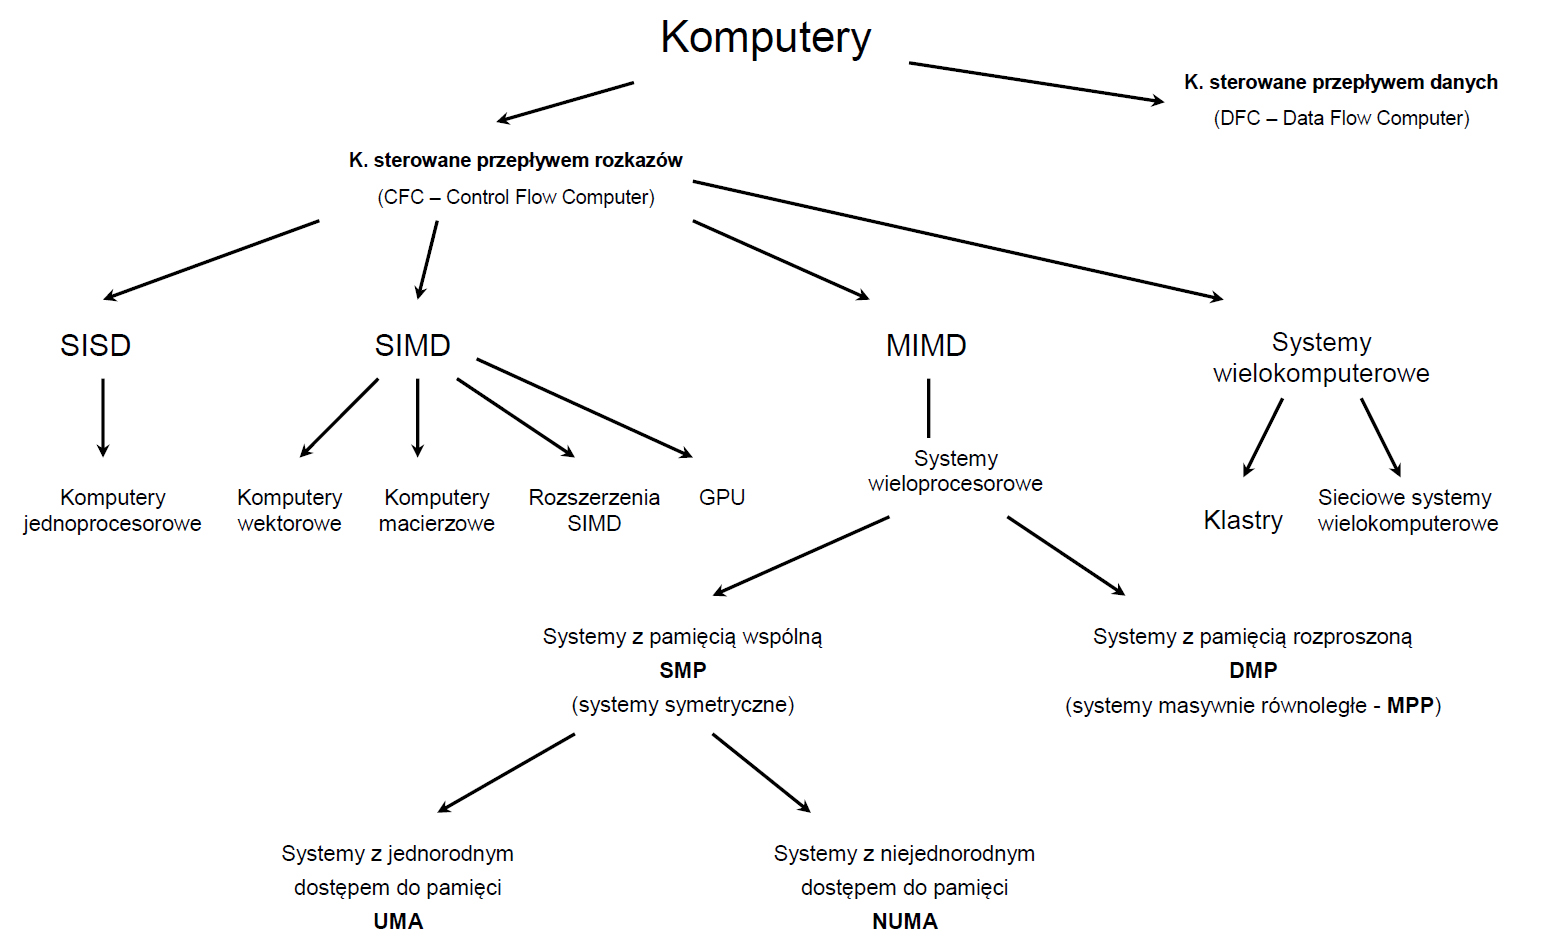
\includegraphics[width=16cm]{klasyfikacja}
\pagebreak
	
\section{Architektura SIMD}
	\subsection{Co to jest?}
		Cecha wyróżniająca dla programisty - rozkazy wektorowe (rozkazy z argumentami wektorowymi).\\
		Dwa różne podejścia do sprzętowej realizacji rozkazów wektorowych:
		\begin{itemize}
			\item Komputery (procesory) macierzowe
			\item Komputery wektorowe
		\end{itemize}
		Idee realizacji obu (macierzowy i wektorowy):\\
		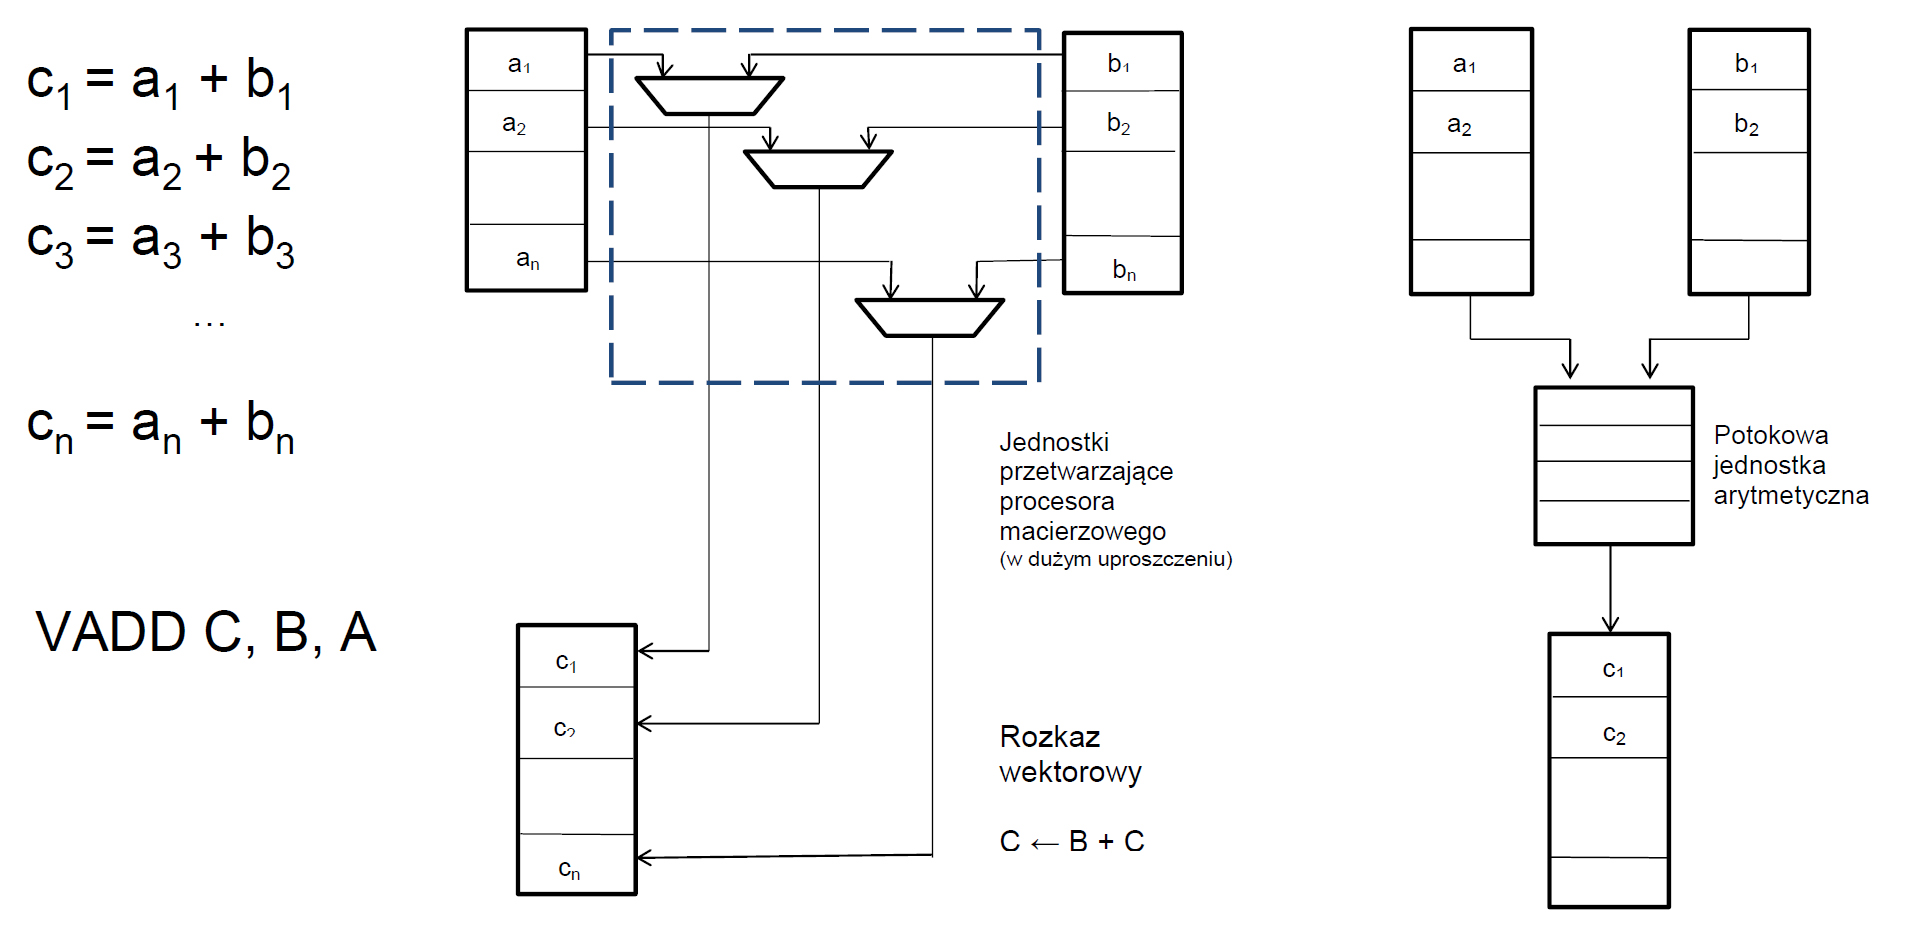
\includegraphics[width=16cm]{wektor_macierz}\\
	\subsection{Komputery wektorowe}
		\subsubsection{Lokalizacja wektorów danych}
			\begin{itemize}
				\item Pamięć operacyjna
				\item Rejestry wektorowe
			\end{itemize}
		\subsubsection{Przykład rozkazu}
			Rozkaz dodawania wektorów: VADDF A,B,C,n\\
			Czas wykonania: $t_{w}=t_{start}+(n-1)\times\tau$\\
			W komputerze macierzowym czas wykonywania tego rozkazu jest równy \emph{const}.
		
		\subsubsection{Przyspieszenie}
			Przyspieszenie jest stosunkiem czasu wykonywania w komputerze klasycznym (szeregowo) do czasu wykonywania w komputerze wektorowym.\\\\
			$a=lim_{n \to \infty}\frac{15\times\tau\times n}{t_{start}+(n-1)\times\tau}=15$
		
		\subsubsection{Przepustowość}
			Przepustowość (moc obliczeniowa) jest stosunkiem ilości operacji zmiennoprzecinkowych do czasu ich wykonania.\\\\
			$Przep=lim_{n \to \infty}\frac{n}{t_{start}+(n-1)\times\tau}=\frac{1}{\tau}$
	
		\subsubsection{Podsumowanie}
			\begin{enumerate}
				\item Hardware
				\begin{itemize}
					\item rozkazy wektorowe
					\item duża liczba potokowych jednostek arytmetycznych
					\item duża liczba rejestrów
				\end{itemize}
				\item Software
				\begin{itemize}
					\item klasyczne języki: Fortran, C
					\item klasyczne algorytmy
					\item kompilatory wektoryzujące
				\end{itemize}
			\end{enumerate}

		\subsubsection{Zastosowanie}
			\begin{itemize}
				\item Numeryczna symulacja ośrodków ciągłych
				\item Równania różniczkowe, równania różnicowe, układy równań algebraicznych (rachunek macierzowy)
				\item Dziedziny zastosowań:
				\begin{itemize}
					\item prognozowanie pogody
					\item symulacja aerodynamiczna
					\item sejsmiczne poszukiwania ropy naftowej i innych surowców
					\item symulacja reakcji jądrowych
					\item medycyna i farmacja
					\item obliczenia inżynierskie dużej skali
				\end{itemize}
			\end{itemize}
		
	\subsection{Komputery macierzowe}
		\subsubsection{Co to jest?}
			Architektura komputerów macierzowych - model SIMD w dwóch wariantach:
			\begin{itemize}
				\item SIMD - DM (z pamięcią rozproszoną)
				\item SIMD - SM (z pamięcią wspólną)
			\end{itemize}
		
		\subsubsection{Elementy komputera macierzowego}
			\begin{enumerate}
				\item \textbf{Jednostka sterująca} - procesor wykonujący rozkazy sterujące i skalarne oraz inicjujący wykonanie rozkazów wektorowych w sieci elementów przetwarzających.
				\item \textbf{Elementy przetwarzające} (procesorowe) - jednostki arytmetyczno-logiczne wykonujące operacje elementarne rozkazów wektorowych.
				\item \textbf{Sieć łącząca} - łączy elementy przetwarzające między sobą lub z modułami pamięci operacyjnej; warianty:
				\begin{itemize}
					\item sieć statyczna: pierścień, gwiazda, krata, drzewo, hipersześcian
					\item sieć dynamiczna: jednostopniowa, wielostopniowa
				\end{itemize}
			\end{enumerate}
		
		\subsubsection{Podsumowanie}
			\begin{itemize}
				\item Architektura SIMD
				\item Jednostka sterująca + jednostka macierzowa
				\item Rozkazy wektorowe - wykonywane synchronicznie w sieci (macierzy) EP
				\item Skomplikowana wymiana danych między EP
				\item Trudne programowanie - konieczność tworzenia nowych wersji algorytmów
			\end{itemize}
		
	\subsection{Model SIMD w procesorach superskalarnych}
		\subsubsection{Technologia MMX}
			\begin{itemize}
				\item 8 rejestrów 64-bitowych MMX
				\item Nowe typy danych
				\item Rozszerzony zestaw instrukcji (57 instrukcji)
				\item Realizacja operacji na krótkich wektorach wg modelu SIMD
			\end{itemize}
	\subsection{Technologia SSE}
		\begin{itemize}
			\item 8 rejestrów 128-bitowych
			\item Osiem 16-bitowych argumentów (elementów wektora) typu integer
			\item Cztery 32-bitowe argumenty integer/fplub dwa 64-bitowe
			\item Operacje zmp na 4-elementowych wektorach liczb 32-bit (pojed. prec.)
		\end{itemize}
		
\section{Karty graficzne i architektura CUDA}
	\subsection{Charakterystyka}
		\begin{itemize}
			\item GPU - Graphics Processing Unit
			\item Wcześniejsze GPU - specjalizowane języki (HLSL, GLSL czy NVIDIA Cg), tylko rendering
			\item CUDA (Compute Unified Device Architecture) -architektura wielordzeniowych procesorów graficznych (GPU)
			\item Uniwersalna architektura obliczeniowa połączona z równoległym modelem programistycznym
			\item wsparcie dla języków C/C++
			\item GPGPU = GPU + CUDA
			\item CUDA - obsługiwana przez karty graficzne GeForce i GeForce Mobile od serii 8 (GeForce 8800), nowsze układy z rodzin Tesla i Quadro, Fermi, obecnie Kepler
		\end{itemize}
	\subsection{Architektura CUDA}
		\begin{itemize}
			\item W miejsce oddzielnych potoków przetwarzających wierzchołki i piksele wprowadzenie uniwersalnego procesora przetwarzającego wierzchołki, piksele i ogólnie geometrię, a także uniwersalne programy obliczeniowe
			\item Wprowadzenie procesora wątków eliminującego „ręczne” zarządzanie rejestrami wektorowymi
			\item Wprowadzenie modelu SIMT (single-instruction multiple-thread), w którym wiele niezależnych wątków wykonuje równocześnie tę samą instrukcję
			\item Wprowadzenie współdzielonej pamięci oraz mechanizmów synchronizacji wątków (barrier synchronization) dla komunikacji między wątkami
		\end{itemize}
	\subsection{Multiprocesor strumieniowy}
		\begin{itemize}
			\item 8 rdzeni C1 -C8 (SP)
			\item podręczna pamięć instrukcji (ang. instruction cache),
			\item podręczna pamięć danych (ang. constant cache) -pamięć tylko do odczytu,
			\item pamięć współdzielona (ang. shared memory)
			\item 16 384 rejestry,
			\item jednostka arytmetyczna wykonująca obliczenia zmiennoprzecinkowe podwójnej precyzji (fp64),
			\item dwie jednostki arytmetyczne przeznaczone do obliczania funkcji specjalnych (ang. special function unit),
			\item pamięć globalna
		\end{itemize}
	\subsection{Model programistyczny CUDA}
		\begin{itemize}
			\item Specjalny kompilator NVCC
			\item Podział programu na kod wykonywany przez procesor (ang. Host code) i przez urządzenie (kartę graficzną) (ang. Device code) - kernel
			\item Realizacja operacji równoległych według modelu SIMT (Single Instruction Multiple Threading)
		\end{itemize}
	\subsection{Wykonanie obliczeń z użyciem architektury CUDA (5 faz)}
		\begin{enumerate}
			\item Przydzielenie w pamięci globalnej obszaru pamięci dla danych, na których będą wykonywane obliczenia przez kernel.
			\item Przekopiowanie danych do przydzielonego obszaru pamięci.
			\item Zainicjowanie przez CPU obliczeń wykonywanych przez GPU, tj. wywołanie kernela.
			\item Wykonanie przez wątki (z użyciem GPU) obliczeń zdefiniowanych w kernelu.
			\item Przekopiowanie danych z pamięci globalnej do pamięci operacyjnej.
		\end{enumerate}
	\subsection{CUDA procesor (rdzeń)}
		\begin{itemize}
			\item Potokowa jednostka arytmetyczna zmp
			\item Potokowa jednostka arytmetyczna stp
			\item Ulepszona realizacja operacji zmp FMA (fused multiply-add) dla pojedynczej i podwójnej precyzji
		\end{itemize}

	\pagebreak
	\section{Wątki}
		\begin{itemize}
			\item Wątek reprezentuje pojedynczą operację (a single work unit or operation)
			\item Wątki są automatycznie grupowane w bloki, maksymalny rozmiar bloku = 512 wątków (w architekturze Fermi i wyższych –1024 wątki).
			\item Bloki grupowane są w siatkę (grid -kratę)
			\item Grupowanie wątków –bloki o geometrii 1, 2 lub 3-wymiarowej
			\item Grupowanie bloków –siatka (grid) o geometrii 1, 2-wymiarowej
			\item Wymaga się, aby bloki wątków tworzących siatkę mogły się wykonywać niezależnie: musi być możliwe ich wykonanie w dowolnym porządku, równolegle lub szeregowo.
		\end{itemize}
		\subsection{Grupowanie wątków w bloki i siatkę}
			\begin{itemize}
				\item Siatka o geometrii jednowymiarowej (trzy bloki wątków)
				\item Każdy blok -geometria dwuwymiarowa (wymiary 2 x 3)
			\end{itemize}
		\subsection{Sprzętowa organizacja wykonywania wątków}
			\begin{itemize}
				\item Przy uruchomieniu kernel’awszystkie bloki tworzące jego siatkę obliczeń są rozdzielane pomiędzy multiprocesory danego GPU
				\item Wszystkie wątki danego bloku są przetwarzane w tym samym multiprocesorze
				\item W danej chwili (cyklu) pojedynczy rdzeń multiprocesora wykonuje jeden wątek programu
				\item Multiprocesor tworzy, zarządza, szereguje i wykonuje wątki w grupach po 32, nazywanych wiązkami (warp).
				\item Wiązki są szeregowane do wykonania przez warp scheduler. Wiązka wątków jest wykonywana jako jeden wspólny rozkaz (analogia do rozkazu SIMD, tzn. rozkazu wektorowego)
				\item Sposób wykonania wiązki wątków (rozkazu SIMD) zależy od budowy multiprocesora:
				\begin{itemize}
					\item Dla architektury Fermi (32 procesory w jednym multiprocesorze / 2 warp-scheduler’y= 16 procesorów na 1 wiązkę) wiązka jest wykonywana jako 2 rozkazy -wiązka jest dzielona na dwie połówki (half –warp) wykonywane jako 2 rozkazy (te same, ale na dwóch zestawach danych).
					\item Dla architektury Tesla (8 procesorów w jednym multiprocesorze, 1 warp-scheduler) wiązka jest dzielona na cztery ćwiartki (quarter-warp) wykonywane jako 4 kolejne rozkazy (te same, ale na czterech zestawach danych).
				\end{itemize}
				\item Konstrukcja warp scheduler’a umożliwia uruchomienie wielu wiązek wątków współbieżnie - warp scheduler pamięta wtedy adresy wiązek, przypisane im rozkazy SIMD oraz ich stan (gotowość do wykonania lub stan oczekiwania na pobranie danych z pamięci).
				\item Współbieżne uruchomienie wielu wiązek pozwala zmniejszyć straty związane z oczekiwaniem na dane (zwykle długi czas dostępu do pamięci).
			\end{itemize}
			
\section{Rodzaje pamięci multiprocesora}
	\begin{itemize}
		\item \textbf{pamięć globalna} – duża pamięć, o czasie życia aplikacji (dane umieszczone w tej pamięci są usuwane po zakończeniu aplikacji), dostępna dla każdego wątku w dowolnym bloku, ale o dość długim czasie dostępu wynoszącym ok. 400-600 taktów zegara,
		\item \textbf{pamięć współdzielona} – niewielka pamięć o czasie życia bloku (zakończenie działania bloku powoduje usunięcie danych w niej przechowywanych), dostępna dla każdego wątku w bloku dla którego jest dedykowana, o bardzo krótkim czasie dostępu,
		\item \textbf{pamięć stałych} – niewielki fragment pamięci globalnej, który jest cache-owany, przez co dostęp do niego jest bardzo szybki. Jest ona tylko do odczytu. Czas życia pamięci stałych oraz jej dostępność jest taka sama jak pamięci globalnej,
		\item \textbf{rejestry} – niewielka, bardzo szybka pamięć o czasie życia wątku (po zakończeniu wątku dane z rejestrów są usuwane). Tylko jeden wątek może w danym momencie korzystać z danego rejestru,
		\item \textbf{pamięć lokalna i pamięć tekstur} – podobnie jak w przypadku pamięci stałych, są to dedykowane fragmenty pamięci globalnej. Pamięć lokalna jest wykorzystywana do przechowywania danych lokalnych wątku, które nie mieszczą się w rejestrach, a pamięć tekstur posiada specyficzne metody adresowania i cache-owanie specyficzne dla zastosowań graficznych.
	\end{itemize}
	
\section{Systemy wieloprocesorowe}
	\subsection{Rodzaje}
		\begin{itemize}
			\item systemy z pamięcią wspólną
			\item systemy z pamięcią rozproszoną
		\end{itemize}
		\subsubsection{Z pamięcią wspólną}
			\begin{itemize}
				\item Systemy z jednorodnym dostępem do pamięci (UMA – Uniform Memory Access)
				\item Systemy z niejednorodnym dostępem do pamięci (NUMA – Non 	- Uniform Memory Access)
				\item Klasyfikacja:
				\begin{itemize}
					\item Systemy ze wspólną magistralą
					\item Systemy wielomagistralowe
					\item Systemy z przełącznicą krzyżową
					\item Systemy z wielostopniową siecią połączeń
					\item Systemy z pamięcią wieloportową
					\item Systemy z sieciami typu punkt - punkt
				\end{itemize}
			\end{itemize}
		\subsubsection{Systemy ze wspólną magistralą}
			\begin{itemize}
				\item prostota konstrukcji – niska złożoność układowa całości
				\item niski koszt
				\item łatwość rozbudowy – dołączenia kolejnego procesora, ale tylko w ograniczonym zakresie
				\item ograniczona złożoność magistrali (jej szybkość jest barierą)
				\item niska skalowalność
			\end{itemize}
	\subsection{Skalowalność}
		\textbf{System skalowalny} - System, w którym dodanie pewnej liczby procesorów prowadzi do proporcjonalnego przyrostu mocy obliczeniowej.
	\subsection{Protokół MESI}
		\begin{itemize}
			\item I - invalid
			\item S - shared
			\item E - exclusive
			\item M - modified
		\end{itemize}
	\subsection{Systemy wielomagistralowe}
		\begin{itemize}
			\item Wielokrotnie zwiększona przepustowość
			\item Konieczność stosowania układu arbitra do sterowania dostępem do magistral
			\item Rozwiązania kosztowne
			\item Zadania każdego przełącznika
			\begin{itemize}
				\item Rozwiązywanie konfliktów dostępu do tego samego modułu pamięci
				\item Zapewnienie obsługi równoległych transmisji, krzyżujących się w przełączniku
			\end{itemize}
		\end{itemize}
	\subsection{Systemy UMA}
		\begin{itemize}
			\item Symetryczna architektura – jednakowy dostęp procesorów do pamięci operacyjnej oraz we/wy
			\item Utrzymanie spójności pamięci podręcznych (cache):
			\begin{itemize}
				\item snooping - metoda starsza i mało skalowalna (głównie w systemach ze wspólną magistralą)
				\item katalog - metoda lepiej skalowalna, stosowana razem z sieciami typu punkt - punkt
			\end{itemize}
			\item Łatwe programowanie (realizacja algorytmów równoległych)
			\item Niska skalowalność
		\end{itemize}
	\subsection{Systemy NUMA}
		\begin{itemize}
			\item PaO fizycznie rozproszona, ale logicznie wspólna
			\item Niejednorodny dostęp do pamięci - PaO lokalna, PaO zdalna
			\item Utrzymanie spójności pamięci podręcznych (cache) - katalog
			\item Hierarchiczna organizacja: procesor – węzeł (system UMA) – system NUMA
			\item Zalety modelu wspólnej pamięci dla programowania
			\item Dobra efektywność dla aplikacji o dominujących odczytach z nielokalnej pamięci
			\item Gorsza efektywność dla aplikacji o dominujących zapisach do nielokalnej pamięci
			\item Skalowalność: 1024 – 2560 rdzeni
		\end{itemize}
	\subsection{Systemy SMP}
		\begin{itemize}
			\item Symetryczna architektura – jednakowy dostęp procesorów do pamięci operacyjnej oraz we/wy (na poziomie fizycznych przesyłów –
			tylko w systemach wieloprocesorowe z pamięcią wspólną fizycznie - UMA)
			\item Utrzymanie spójności pamięci podręcznych (cache):
			\begin{itemize}
				\item systemy UMA - snooping lub katalog
				\item systemy NUMA - katalog
			\end{itemize}
			\item Łatwe programowanie (realizacja algorytmów równoległych)
			\item Niska (UMA) i średnia (NUMA) skalowalność
		\end{itemize}

% !TeX spellcheck = pl_PL

%===============================================================================
% *** PYTANIA I ODPOWIEDZI *****************************************************
%===============================================================================
\part{Pytania zamknięte}
\begin{enumerate}
	\question{%
		question={Moc obliczeniowa komputerów wektorowych}%
	}{%
		isTrue1={Nie},%
		answer1={Zależy od liczby stopni potoku.},%
		explain1={Moc obliczeniowa nie jest zależna od liczby stopni potoku. Ta jedynie wpływa na ilosć rozkazów jakie mogą być wykonane w chwili czasu w jednostce potokowej.},%
		isTrue2={Tak},%
		answer2={Jest odwrotnie proporcjonalna do długości taktu zegarowego},%
		explain2={Tak, obliczamy ją wzorem $Przep=lim_{n\to\infty}\frac{n}{t_{start}+(n-1)\times\tau}=\frac{1}{\tau}$},%
		isTrue3={Nie},%
		answer3={Jest wprost proporcjonalna do długości taktu zegarowego},%
		explain3={Nie, patrz wyżej.},%
		isTrue4={Nie},%
		answer4={Zależy odwrotnie proporcjonalnie od liczby jednostek potokowych połączonych łańcuchowo.},%
		explain4={Nie, idea operacji wektorowej na komputerze wektorowym zakłada jedną jednostkę potokową. Ich zwiększenie nie powinno wpłynąć bezpośrednio na moc.},%
		isTrue5={Tak},%
		answer5={Zmierza asymptotycznie do wartości maksymalnej wraz ze wzrostem długości wektora}, %
		explain5={Tak, istnieje pewna wartość maksymalna do której moc dąży logarytmicznie wraz ze wzrostem długości wektora.}, %
		isTrue6={Nie}, %
		answer6={Nie zależy od długości wektora}, %
		explain6={Bzdura, patrz wyżej.}, %
		isTrue7={Nie}, %
		answer7={Zależy liniowo od długości wektora}, %
		explain7={Bzdura, patrz wyżej.}, %
	}
	\question{%
		question={Komputery macierzowe}%
	}{%
		isTrue1={Tak},%
		answer1={Mają w liście rozkazów m.in. rozkazy operujące na wektorach danych},%
		explain1={Tak, te komputery są rozwinięciem komputerów wektorowych i muszą mieć rozkazy wektorowe. Komputery macierzowe posiadają po \emph{n} jednostek przetwarzających, które potrafią razem obliczyć \emph{n} składowych wektora.},%
		isTrue2={Nie},%
		answer2={Mają macierzowe potokowe układy arytmetyczne},%
		explain2={Nie, posiadają natomiast jednostki przetwarzające. Z kolei potokową jednostkę arytmetyczną posiadają komputery wektorowe.},%
		isTrue3={Nie},%
		answer3={Mają w typowych rozwiązaniach zestaw pełnych procesów połączonych siecią połączeń},%
		explain3={Nie, w typowym rozwiązaniu jest jeden pełny procesor z wieloma jednostkami potokowymi, które są połączone siecią łączącą (statyczną lub dynamiczną). Sieć połączeń pełnych procków posiadają superkomputery z top500 (Nie jestem pewien tej odpowiedzi).},%
		isTrue4={Tak},%
		answer4={Wykonują synchroniczną operację wektorową w sieci elementów przetwarzających},%
		explain4={Tak właśnie działają.},%
	}
\begin{minipage}{\textwidth}
	\question{%
		question={Czy poniższa lista jest rosnąco uporządkowana według skalowalności:}%
	}{%
		isTrue1={Nie},%
		answer1={Systemy ściśle połączone, systemy ze wspólną pamięcią, systemy SMP},%
		explain1={Systemy SMP to cała kategoria systemów z pamięcią wspólną, z kolei systemy ściśle połączone i systemy ze wspólną pamięcią są \textbf{równoznaczne} - są przeciwieństwem do systemów luźno powiązanych (z pamięcią rozproszoną).},%
		isTrue2={Tak},%
		answer2={Systemy ze wspólną magistralą, systemy wielomagistralowe, systemy z przełącznicą krzyżową},%
		explain2={Są to systemy wieloprocesorowe (UMA) z pamięcią wspólną, patrz: Klasyfikacja  \ref{subsubsec:klasyfikacjaUMA}\\
			- \emph{Systemy ze wspólna magistralą} - najprostsze i najmniej skalowalne\\
			- \emph{Systemy wielomagistralowe} - szybsze i bardziej złożone, wciąż kiepsko skalowalne\\
			- \emph{Systemy z przełącznicą krzyżową} - duża szybkość i złożoność obliczeniowa, trudne w rozbudowie\\
			Ogółem jest to dolna półka tych systemów.},%
		isTrue3={Nie},%
		answer3={Systemy SMP, systemy z pamięcią wieloportową, systemy z przełącznicą krzyżową},%
		explain3={SMP to rodzaj architektury, z kolei w systemach UMA systemy z przełącznicą krzyżową są mniej skalowalne niż systemy z pamięcią wieloportową, patrz: Klasyfikacja  \ref{subsubsec:klasyfikacjaUMA}.},%
		isTrue4={Nie},%
		answer4={NUMA, MPP, SMP},%
		explain4={MPP jest znacznie bardziej skalowalny niż SMP (pamięć rozproszona $ > $ pamięć wspólna). NUMA to systemy SMP z niejednorodnym dostępem do pamięć - są bardziej skalowalne niż zwykłe SMP (dzięki szybkiej pamięci lokalnej \emph{cache}), ale mniej niż MPP.},%
		isTrue5={Tak},%
		answer5={Systemy z pamięcią wspólną, systemy o niejednorodnym dostępie do pamięci, z pamięcią rozproszoną}, %
		explain5={Dwa pierwsze to rodzaje systemów SMP. Najmniej skalowalne są systemy z pamięcią wspólną, domyślnie o jednorodnym dostępie do pamięci (UMA). Niejednorodny dostęp do pamięci wspólnej (NUMA) jest szybszy, ponieważ wykorzystuje pamięć lokalną procesora, węzły i katalogi. Mechanizm katalogów jest o wiele bardziej skalowalny niż mechanizm "\emph{snoopingu}", wykorzystywany w UMA. Następnie system z pamięcią rozproszoną to MPP - system masywnie równoległy. Jest najbardziej skalowalny ze wszystkich.}, %
		isTrue6={Nie}, %
		answer6={SMP, NUMA, klastry, UMA}, %
		explain6={SMP jest najmniej skalowalny z wymienionych. UMA ma jednorodny dostęp do pamięci i jest mniej skalowalna od NUMA. Klastry są najbardziej skalowalne (nie wiem czy mniej lub bardziej do MPP).}, %
		isTrue7={Tak}, %
		answer7={Systemy symetryczne, o niejednorodnym dostępie do pamięci, systemy z przesyłem komunikatów}, %
		explain7={Systemy symetryczne to SMP z jednorodnym dostępem do pamięci. Systemy SMP z niejednorodnym dostępem są bardziej skalowalne. Z kolei systemy z przesyłem komunikatów sugerują system MPP, z pamięcią rozproszoną - jest on najbardziej skalowalny.}, %
	}
\end{minipage}

\begin{minipage}{\textwidth}
	\question{%
		question={Przetwarzanie potokowe}%
	}{%
		isTrue1={Nie},%
		answer1={Nie jest realizowane dla operacji zmiennoprzecinkowych},%
		explain1={Nie ma takiego ograniczenia. Przetwarzanie potokowe dotyczy optymalizacji czasu wykonywania rozkazów - podziału realizacji rozkazu na fazy. Owszem, dla argumentów zmiennoprzecinkowych mogą wystąpić problemy związane z czasem obliczeń (uniemożliwienie wykonania rozkazu w jednym takcie), co może zablokować napełnianie potoku, jednak nie uniemożliwia to zastosowania potoku.},%
		isTrue2={Nie},%
		answer2={Nie jest realizowane w procesorach CISC},%
		explain2={Przetwarzanie potokowe znalazło zastosowanie głównie w architekturze RISC, jednak CISC też z niej korzysta. Przykłady: VAX 11/780 (CISC), Ultra SPARC III (RISC)},%
		isTrue3={Tak},%
		answer3={Daje przyspieszenie nie większe od liczby segmentów (stopni) jednostki potokowej},%
		explain3={Tak, przyspieszenie jest stosunkiem czasu wykonywania \emph{n} rozkazów dla procesora niepotokowego oraz czasu dla procesora potokowego. W idealnym przypadku, gdy każdy stopień dzieli okres rozkazu po równo, a liczba rozkazów dąży do nieskończoności, stosunek ten jest równy P - ilości stopni.},%
		isTrue4={Nie},%
		answer4={W przypadku wystąpienia zależności między danymi wywołuje błąd i przerwanie wewnętrzne.},%
		explain4={Hm, dobre pytanie. Tak, zależności danych mogą wystąpić (zjawisko hazardu) i rozdupić program, ale po to właśnie istnieją mechanizmy by temu zapobiegać. Każda szanująca się architektura to potrafi: albo sprzętowo, albo na etapie kompilacji, która modyfikuje i optymalizuje program. A jeżeli po modyfikacji pewien rozkaz nie wykona się w jednym takcie, napełnianie potoku jest przerywane (ale błędu chyba nie wywala), patrz wyżej.},%
		isTrue5={Nie},%
		answer5={Jest realizowane tylko dla operacji zmiennoprzecinkowych}, %
		explain5={Pfff, no chyba nie XD Jest realizowane dla każdego rodzaju rozkazu.} %
	}
\end{minipage}
% --- PYTANIE 5
\begin{minipage}{\textwidth}
\question{%
	question={W procesorach superskalarnych}%
}{%
	isTrue1={Tak},%
	answer1={Liczba rozkazów, które procesor może wykonać w 1 takcie zależy od liczby jednostek potokowych w procesorze},%
	explain1={Procesory superskalarne posiadają wiele jednostek potokowych, które są konieczne by móc wykonywać wiele rozkazów w jednym takcie. Od ich liczby zależy owa liczba rozkazów.},%
	isTrue2={Nie},%
	answer2={Liczba rozkazów, które procesor może wykonać w jednym takcie, zależy od liczby stopni potoku.},%
	explain2={Nie, liczba stopni potoku mówi, na ile części dzieli się dany rozkaz w tej jednostce potokowej. One umożliwiają wykonanie wielu rozkazów w jednej jednostce czasu, jednak nie przekłada się to bezpośrednio na liczbę rozkazów, ze względu na zawikłania czasowe, oraz nie jest to idea procesora superskalarnego.},%
	isTrue3={Nie},%
	answer3={Liczba rozkazów pobieranych z pamięci, w każdym takcie musi przekraczać liczbę jednostek potokowych},%
	explain3={Liczba pobranych rozkazów powinna być co najmniej równa ilości jednostek potokowych.},%
	isTrue4={Tak},%
	answer4={Liczba rozkazów, które procesor może wykonać w taktach zależy od liczby jednostek potokowych w procesorze},%
	explain4={Tak, patrz pierwsza odpowiedź.},%
}
\end{minipage}
\begin{minipage}{\textwidth}
	\question{%
		question={Systemy SMP}%
	}{%
		isTrue1={Nie},%
		answer1={Wykorzystują protokół MESI do sterowania dostępem do wspólnej magistrali},%
		explain1={Ten protokół wykorzystują systemy \textbf{UMA} (podkategoria systemów SMP) ze wspólną magistralą w celu zapewnienia spójności pamięci podręcznych (\emph{snooping}). Mogą też używać katalogów, ale podkategoria \textbf{NUMA} wykorzystuje wyłącznie katalogi.},%
		isTrue2={Nie},%
		answer2={Posiadają skalowalne procesory},%
		explain2={SMP należy do systemów wieloprocesorowych, ale te nie muszą być skalowalne.},%
		isTrue3={Nie},%
		answer3={Posiadają pamięć fizycznie rozproszoną, ale logicznie wspólną},%
		explain3={Nie, pamięć jest fizycznie wspólna. Fizycznie rozproszoną pamięć posiadają systemy MPP.},%
	}
\end{minipage}
\begin{minipage}{\textwidth}
	\question{%
		question={Komputery wektorowe}%
	}{%
		isTrue1={Nie},%
		answer1={Posiadają jednostki potokowe o budowie wektorowej},%
		explain1={Nie, posiadają potokowe jednostki arytmetyczne, które nie są wektorowe.},%
		isTrue2={Tak},%
		answer2={Posiadają w liście rozkazów m.in. rozkazy operujące na wektorach danych},%
		explain2={Jak najbardziej, nie mogłyby się bez tego obejść.},%
		isTrue3={Tak},%
		answer3={Wykorzystują od kilku do kilkunastu potokowych jednostek arytmetycznych},%
		explain3={Tak, tych jednostek może być wiele, można to zauważyć na przykładzie komputera Cray-1 (wykład 7-8, slajd 31)},%
		isTrue4={Nie},%
		answer4={Posiadają listę rozkazów operujących wyłącznie na wektorach},%
		explain4={Zdecydowanie nie. Owszem, te komputery posiadają rejestry wektorowe i wektorowe jednostki zmiennoprzecinkowe, ale nie jest to wszystko. Mają również normalne rejestry, adresację, jednostki skalarne i możliwość wykonywania na nich operacji.},%
	}
\end{minipage}
\begin{minipage}{\textwidth}
	\question{%
		question={Procesory wektorowe}%
	}{%
		isTrue1={Tak},%
		answer1={Mogą być stosowane w systemach wieloprocesorowych},%
		explain1={Domyślnie procesory wektorowe mogą pracować pojedynczo, ale mogą być częścią takiego systemu. Poza tym nie znalazłem nic, co by temu przeczyło. Jest też np. CUDA - architektura wielordzeniowych procesorów graficznych. Sama architektura SIMD działa na wielu procesorach.},%
		isTrue2={Nie},%
		answer2={Mają listę rozkazów operującą jedynie na wektorach},%
		explain2={Nie, posiadają też m.in. potokowe jednostki arytmetyczne oraz jednostki skalarne, do operowania na zwykłych liczbach.},%
		isTrue3={Tak},%
		answer3={Mają moc kilka razy większą od procesorów skalarnych},%
		explain3={Tak, przyspieszenie jest ilorazem czasu wykonywania na procesorze niewektorowym do czasu wykonywania na procesorze wektorowym. Np. dla rozkazu dodawania \emph{n} wektorów przyspieszenie wyliczane jest wg wzoru $ a=\frac{15\tau n}{t_{start}+(n-1)\tau} $, gdzie przy \emph{n} dążącym do nieskończoności \emph{a} jest równe 15.},%
	}
\end{minipage}
\begin{minipage}{\textwidth}
	\question{%
		question={Systemy MPP są zbudowane z węzłów którymi mogą być}%
	}{%
		isTrue1={Tak},%
		answer1={Systemy SMP},%
		explain1={Węzłami mogą być zarówno systemy UMA, jak i NUMA. Ponadto dopuszcza się zwykłe procesory z pamięcią operacyjną. Patrz: organizacja MPP \ref{subsec:organizacjaMPP}. Są to \textbf{jedyne} możliwe rodzaje węzłów.},%
		isTrue2={Nie},%
		answer2={Klastry},%
		explain2={Patrz wyżej.},%
		isTrue3={Nie},%
		answer3={Konstelacje},%
		explain3={Patrz wyżej.},%
		isTrue4={Tak},%
		answer4={Systemy NUMA},%
		explain4={Patrz wyżej.},%
		isTrue5={Tak},%
		answer5={Procesory}, %
		explain5={Patrz wyżej.}, %
	}
\end{minipage}
\begin{minipage}{\textwidth}
	% --- PYTANIE 10
	\question{%
		question={W architekturze NUMA}%
	}{%
		isTrue1={Tak},%
		answer1={Dane są wymieniane między węzłami w postaci linii pamięci podręcznej (PaP)},%
		explain1={Tak, każdy procesor / węzeł posiada swoją własną szybką pamięć podręczną. Pamięć ta jest publiczna - inne procesory mają do niej dostęp, ale wymiana informacji na linii \emph{moja pamięć - inny procesor} jest znacznie wolniejsza niż \emph{procesor - jego pamięć}.},%
		isTrue2={Nie},%
		answer2={Spójność PaP węzłów jest utrzymywana za pomocą protokołu MESI},%
		explain2={Protokół MESI jest wykorzystywany w architekturze \textbf{UMA} do \emph{snoopingu} - zapewnienia spójności pamięci podręcznych procków.},%
		isTrue3={Nie},%
		answer3={Czas dostępu do pamięci lokalnej w węźle jest podobny do czasu dostępu do pamięci nielokalnej},%
		explain3={Odwołanie do nielokalnej pamięci są znacznie wolniejsze niż do lokalnej, ok. 10-krotnie bardziej. Dotyczy to głównie architektury NC-NUMA, patrz: rodzaje systemów NUMA \ref{subsec:rodzajeNUMA}},%
		isTrue4={Tak},%
		answer4={Czas zapisu danych do pamięci nielokalnej może być znacznie dłuższy od czasu odczytu z tej pamięci},%
		explain4={Patrz wyżej.},%
		isTrue5={Tak},%
		answer5={Każdy procesor ma dostęp do pamięci operacyjnej każdego węzła}, %
		explain5={Patrz wyżej.}, %
		isTrue6={Nie}, %
		answer6={Procesy komunikują się poprzez przesył komunikatów}, %
		explain6={Przesył komunikatów występuje w systemach MPP, gdzie pamięć jest rozproszona fizycznie i logicznie. W NUMA jest fizycznie rozproszona między węzłami (do przesyłu informacji wykorzystywana jest sieć łączącą węzły), ale stanowi logicznie jedną całość.}, %
		isTrue7={Tak}, %
		answer7={Pamięć operacyjna jest rozproszona fizycznie pomiędzy węzłami, ale wspólna logicznie}, %
		explain7={Patrz wyżej.}, %
	}
\end{minipage}
\begin{minipage}{\textwidth}
	\question{%
		question={Mechanizmy potokowe stosowane są w celu}%
	}{%
		isTrue1={Nie},%
		answer1={Uszeregowania ciągu wykonywanych rozkazów},%
		explain1={Nie, zupełnie nie o to chodzi. Ciąg może zostać uszeregowany przez kompilator w celu optymalizacji. Jednak celem tego mechanizmu jest zrównoleglenie wykonywania rozkazów $ \rightarrow $ zmiana kolejności ich realizacji nie jest założeniem.},%
		isTrue2={Tak},%
		answer2={Uzyskania równoległej realizacji rozkazów},%
		explain2={No tyć. Potoki umożliwiają realizację wielu rozkazów jednocześnie dzieląc jednostkę centralną na wg stopni, jak np. pobranie rozkazu i wykonania rozkazu. Dzięki temu dwa rozkazy mogą wykonywać się jednocześnie, oba w innych fazach (jednostkach czasu).},%
		isTrue3={Tak},%
		answer3={Przyspieszenia realizacji rozkazów},%
		explain3={Tak, to główny cel. Umożliwienie wykonania rozkazów umożliwia przyspieszenie, które oblicza się jako stosunek czasu wykonywania rozkazów w procesorze niepotokowym do czasu realizacji w procesorze potokowym. W idealnym przypadku jest ono równe \emph{P} - ilości podziałów / stopni / faz / zwał jak zwał.},%
	}
\end{minipage}
\begin{minipage}{\textwidth}
	\question{%
		question={Protokół MESI}%
	}{%
		isTrue1={Nie},%
		answer1={Jest wykorzystywany do sterowania dostępem do magistrali w systemie SMP},%
		explain1={Protokół MESI wykorzystywany jest do zapewniania spójności pamięci podręcznych \emph{cache} w architekturze SMP (\emph{snooping}), a dokładniej w UMA. NUMA korzysta tylko z katalogów.},%
		isTrue2={Tak},%
		answer2={Zapewnia spójność pamięci cache w systemie SMP},%
		explain2={Do tego właśnie służy.},%
		isTrue3={Nie},%
		answer3={Służy do wymiany komunikatów w systemie MPP},%
		explain3={Patrz wyżej.},%
		isTrue4={Nie},%
		answer4={Chroni przed hazardem w procesorach superskalarnych},%
		explain4={Patrz wyżej.},%
	}
\end{minipage}
\begin{minipage}{\textwidth}
	\question{%
		question={Mechanizm skoków opóźnionych}%
	}{%
		isTrue1={Tak},%
		answer1={Polega na opóźnianiu wykonywania skoku do czasu wykonania rozkazu następnego za skokiem},%
		explain1={Tak, cały ten mechanizm sprowadza się do opóźnienia efektu skoku o jeden rozkaz. Zapewnia to, że rozkaz następny po skoku zawsze będzie wykonywany w całości.},%
		isTrue2={Nie},%
		answer2={Wymaga wstrzymania potoku na jeden takt.},%
		explain2={Nie, mechanizm potoków nie musi być wstrzymywany. Mechanizm ten zmienia postać programu w trakcie kompilacji, ale na samą realizację potoku nie ma wpływu (afaik, not sure).},%
		isTrue3={Nie},%
		answer3={Powoduje błąd na końcu pętli},%
		explain3={Pfff, jak programista ssie pałę to tak, jednak w założeniu tak się nie dzieje.},%
		isTrue4={Tak},%
		answer4={Wymaga umieszczenia rozkazu NOP za rozkazem skoku lub reorganizacje programu},%
		explain4={Tak, mechanizm sprowadza się do tego, i tylko do tego, patrz pierwsza odpowiedź.},%
	}
\end{minipage}
\begin{minipage}{\textwidth}
	\question{%
		question={Charakterystyczne cechy architektury MPP}%
	}{%
		isTrue1={Nie},%
		answer1={Spójność pamięci podręcznej wszystkich węzłów},%
		explain1={},%
		isTrue2={Tak},%
		answer2={Fizycznie rozproszona PaO},%
		explain2={},%
		isTrue3={Nie},%
		answer3={Fizycznie rozproszona PaO, ale logicznie wspólna},%
		explain3={},%
		isTrue4={Tak},%
		answer4={Przesył komunikatów między procesorami},%
		explain4={},%
		isTrue5={Nie},%
		answer5={Niska skalowalność}, %
		explain5={}, %
		isTrue6={Nie}, %
		answer6={Jednorodny dostęp do pamięci wszystkich węzłów}, %
		explain6={}, %
	}
\end{minipage}

% --- PTYTANIE 15
\question{%
	question={Jak można ominąć hazard danych}%
}{%
isTrue1={Nie},%
answer1={Poprzez rozgałęzienia},%
explain1={Nie, rozgałęzienie to po prostu instrukcje typu IF, które tworzą takie rozgałęzienia. Mechanizm przewidywania rozgałęzień jest stosowany do usuwania hazardu sterowania związanego ze skokami i rozgałęzieniami.},%
isTrue2={Nie},%
answer2={Poprzez uproszczenie adresowania - adresowanie bezpośrednie.},%
explain2={Bullshit. Nie wiem w czym miało by pomóc uproszczenia adresowania, poza pójściem w stronę RISCu, ale na hazard to nie pomoże. Tym można tylko skrócić czas odwołania się do danych.},%
isTrue3={Tak},%
answer3={Przez zamianę rozkazów},%
explain3={Tak, i na tym polega mechanizm skoków opóźnionych, które mogą program zmodyfikować (dodać rozkaz NOP) albo zoptymalizować, właśnie zamieniają rozkazy kolejnością.},%
}


\question{%
	question={Cechy architektury CISC}%
}{%
isTrue1={Nie},%
answer1={Czy może być wykonana w VLIW},%
explain1={Nie, architektura VLIW dotyczy mikroprocesorów i miała na celu jak największe zmniejszenie jednostki centralnej i jej rozkazów (RISC).},%
isTrue2={Tak},%
answer2={Czy występuje model wymiany danych typu pamięć - pamięć},%
explain2={Tak, posiada również niewielką ilość rejestrów.},%
isTrue3={Nie},%
answer3={Jest mała liczba rozkazów},%
explain3={Nie, w tej architekturze jest PEŁNA (complex) lista rozkazów. Niektóre z zaawansowanych pleceń nawet nie były wykorzystywane, i bum! tak powstał RISC.},%
}


\question{%
	question={Cechy architektury RISC}%
}{%
isTrue1={Tak},%
answer1={Czy występuje model wymiany danych typu rej-rej},%
explain1={Tak, a komunikacja z pamięcią operacyjną odbywa się wyłącznie za pomocą rozkazów LOAD i STORE.},%
isTrue2={Tak},%
answer2={Jest mała liczba trybów adresowania},%
explain2={Tak, raptem 4 w procesorze RISC I podczas gdy CISCi mogą mieć ich kilkanaście, w tym takie bardzo złożone.},%
isTrue3={Nie},%
answer3={Jest wykonywanych kilka rozkazów w jednym takcie},%
explain3={Fałsz. Prawdziwe wykonywanie wielu rozkazów w jednym takcie wymaga superskalarnosci - wielu jednostek potokowych. Cechą architektury RISC jest potokowość, ale pojedyncza.},%
isTrue4={Tak},%
answer4={Jest wykonywanych kilka rozkazów w jednym takcie (w danej chwili czasu)},%
explain4={Chodzi o przetwarzanie potokowe. Tu jest haczyk - pierwszy procesor RISC I (1980) stawiał sobie za cel wykonanie \emph{jednego rozkazu w jednym takcie} i dokładnie tak brzmiało jego założenie projektowe. Jednak jego fizyczna realizacja (1982) posiadała dwustopniowy potok. Również w wykładach jako cecha tej architektury jest napisane "Intensywne wykorzystanie przetwarzania potokowego", co odnosi się do faktu, że obecnie nie ma procesora typu RISC, który go nie ma. Wg mnie prawda.},%
isTrue5={Nie},%
answer5={Jest wykonywanych kilka instrukcji procesora w jednym rozkazie asemblerowym}, %
explain5={Nic mi na ten temat nie wiadomo. Brzmi jednak zbyt hardo i odlegle od tematu zmniejszania ilości rozkazów.}, %
isTrue6={Tak}, %
answer6={Układ sterowania w postaci logiki szytej}, %
explain6={Tak.}, %
}


\question{%
	question={Przepustowość (moc obliczeniowa) dużych komputerów jest podawana w:}%
}{%
isTrue1={Tak},%
answer1={GFLOPS},%
explain1={},%
isTrue2={Nie},%
answer2={Liczbie instrukcji wykonywanych na sekundę},%
explain2={},%
isTrue3={Tak},%
answer3={Liczbie operacji zmiennoprzecinkowych na sekundę},%
explain3={},%
isTrue4={Nie},%
answer4={Mb/sek},%
explain4={To jest do zapamiętania na prostu - takie są standardy},%
}


\question{%
	question={Podstawą klasyfikacji Flynna jest}%
}{%
isTrue1={Nie},%
answer1={Liczba jednostek przetwarzających i sterujących w systemach komputerowych},%
explain1={},%
isTrue2={Nie},%
answer2={Protokół dostępu do pamięci operacyjnej},%
explain2={},%
isTrue3={Nie},%
answer3={Liczba modułów pamięci operacyjnej w systemach komputerowych},%
explain3={},%
isTrue4={Tak},%
answer4={Liczba strumieni rozkazów i danych w systemach komputerowych},%
explain4={To po prostu należy zapamiętać. \textbf{Kryterium klasyfikacji Flynna jest \emph{liczba strumieni rozkazów} oraz \emph{liczba strumieni danych} w systemie komputerowym. NIC WIĘCEJ, NIC MNIEJ.\\Albo inaczej: \emph{$Liczba\_strumieni\times(rozkazow+danych)$}}},%
}


% --- PYTANIE 20
\question{%
	question={Rozkazy wektorowe mogą być realizowane przy wykorzystaniu}%
}{%
isTrue1={Tak},%
answer1={Macierzy elementów przetwarzających},%
explain1={Tak, komputery macierzowe operują na rozkazach wektorowych.},%
isTrue2={Nie},%
answer2={Zestawu procesorów superskalarnych},%
explain2={Procesory superskalarne w założeniu nie posiadają rozkazów wektorowych.},%
isTrue3={Tak},%
answer3={Technologii MMX},%
explain3={Tak, jest to pochodna technologia modelu SIMD, wykonuje operacje na krótkich wektorach (64-bit)},%
isTrue4={Nie},%
answer4={Sieci połączeń typu krata},%
explain4={Jest to sieć połączeń, która łączy jednostki przetwarzające w komputerze macierzowym. Raczej na wektorach na częsć komputera nie działa.},%
isTrue5={Tak},%
answer5={Potokowych jednostek arytmetycznych}, %
explain5={Tak, takie znajdują się w komputerach wektorowych.}, %
}


\question{%
	question={Architektura superskalarna}%
}{%
isTrue1={Nie},%
answer1={Dotyczy systemów SMP},%
explain1={Zdecydowanie nie tylko. Architektura superskalarna wymaga mechanizmu potokowego, czyli dotyczy głównie architektury RISC.},%
isTrue2={Nie},%
answer2={Wymaga zastosowania protokołu MESI},%
explain2={Nie, architektura superskalarna wymaga jedynie zastosowania co najmniej dwóch jednostek potokowych.},%
isTrue3={Tak},%
answer3={Umożliwia równoległe wykonywanie kilku rozkazów w jednym procesorze},%
explain3={Tak, i taki jest cel jej istnienia. Umożliwia to mechanizm potokowy.},%
isTrue4={Nie},%
answer4={Wywodzi się z architektury VLIW},%
explain4={Wręcz odwrotnie, to VLIW wykorzystuje architekturę superskalarną na której opiera swój podział rozkazów na paczki.},%
}


\question{%
	question={Klastry}%
}{%
isTrue1={Nie},%
answer1={Mają średnią skalowalność},%
explain1={},%
isTrue2={Nie},%
answer2={Wykorzystują model wspólnej pamięci},%
explain2={},%
isTrue3={Tak},%
answer3={W węzłach mogą wykorzystywać systemy SMP},%
explain3={},%
isTrue4={Tak},%
answer4={Do komunikacji między procesami wykorzystują przesył komunikatów},%
explain4={},%
isTrue5={Nie},%
answer5={Wykorzystują przełącznicę krzyżową jako sieć łączącą węzły}, %
explain5={}, %
isTrue6={Tak}, %
answer6={W każdym węźle posiadają pełną instalację systemu operacyjnego}, %
explain6={}, %
}


\question{%
	question={Pojęcie równoległości na poziomie rozkazów}%
}{%
isTrue1={Nie},%
answer1={Dotyczy architektury MIMD},%
explain1={Nie, ten rodzaj równoległości dotyczy mechanizmów potokowych (CISC i RISC), architektury superskalarnej oraz VLIW.},%
isTrue2={Tak},%
answer2={Odnosi się m.in. do przetwarzania potokowego},%
explain2={Tak, ideą mechanizmu potoków jest zrównoleglenie rozkazów i możliwość wykonywania wielu z nich w tej samej chwili czasu.},%
isTrue3={Nie},%
answer3={Dotyczy architektury MPP},%
explain3={Nie, patrz wyżej.},%
isTrue4={Tak},%
answer4={Dotyczy m.in. architektury superskalarnej},%
explain4={Tak, patrz wyżej.},%
}


\question{%
	question={Systemy wieloprocesorowe z pamięcią wspólną}%
}{%
isTrue1={Nie},%
answer1={Zapewniają jednorodny dostęp do pamięci},%
explain1={},%
isTrue2={Tak},%
answer2={Mogą wykorzystywać procesory CISC},%
explain2={},%
isTrue3={Tak},%
answer3={Są wykorzystywane w klastrach},%
explain3={},%
isTrue4={Nie},%
answer4={Wykorzystują przesył komunikatów między procesorami},%
explain4={},%
isTrue5={Tak},%
answer5={Wykorzystują katalog do utrzymania spójności pamięci podręcznych}, %
explain5={}, %
}


% --- PYTANIE 25
\question{%
	question={Hazard danych}%
}{%
isTrue1={Tak},%
answer1={Czasami może być usunięty przez zmianę kolejności wykonania rozkazów},%
explain1={Tak, służy do tego mechanizm skoków opóźnionych, który odbywa się na poziomie kompilacji programu.},%
isTrue2={Nie},%
answer2={Nie występuje w architekturze superskalarnej},%
explain2={Występuje wszędzie tam gdzie jest potokowe przetwarzania rozkazów.},%
isTrue3={Nie},%
answer3={Jest eliminowany przez zastosowanie specjalnego bitu w kodzie program},%
explain3={Nic mi o tym nie wiadomo. Pewne dodatkowe bity są wykorzystywane w mechanizmie przewidywania rozgałęzień, który służy do eliminacji hazardu, jednak on to odbywa się PRZED realizacją programu i sprowadza się do zmiany kolejnosci wykonywania rozkazów przez kompilator. Nic nie dodaje do treści programu.},%
isTrue4={Nie},%
answer4={Może wymagać wyczyszczenia potoku i rozpoczęcia nowej (...)},%
explain4={Nie wiem jak hazard danych może czegokolwiek wymagać skoro jest zjawiskiem ubocznym i je eliminujemy. Sprzętowa i programowa eliminacja hazardu jedynie może doprowadzić do \textbf{wstrzymania} napełniania potoku.},%
}


\question{%
	question={Przetwarzanie wielowątkowe}%
}{%
isTrue1={Tak},%
answer1={Zapewnia lepsze wykorzystanie potoków},%
explain1={Tak, ma na celu minimalizację strat cykli w trakcie realizacji wątku, jakie mogą powstać na wskutek:\\ - chybionych odwołań do pamięci podręcznej;\\- błędów w przewidywaniu rozgałęzień;\\- zależności między argumentami},%
isTrue2={Tak},%
answer2={Minimalizuje straty wynikające z chybionych odwołań do pamięci podręcznej},%
explain2={Tak, patrz wyżej.},%
isTrue3={Tak},%
answer3={Wymaga zwielokrotnienia zasobów procesora (rejestry, liczniki rozkazów, itp.)},%
explain3={Niestety tak, jest to warunek sprzętowej realizacji wielowątkowości.},%
isTrue4={Nie},%
answer4={Nie może być stosowane w przypadku hazardu danych},%
explain4={Nie, hazard danych wynika z zależności między argumentami, które są naturalnym ryzykiem przy stosowaniu mechanizmu potokowego. Nie powinny być blokowane z tego powodu, tym bardziej, że wielowątkowość ma dodatkowo chronić liczbę cykli przed zgubnym wpływem hazardu.}, %
}


\question{%
	question={Okna rejestrów}%
}{%
isTrue1={Nie},%
answer1={Chronią przez hazardem danych},%
explain1={Lolnope, od tego są mechanizmy skoków opóźnionych i przewidywania rozgałęzień. Okno rejestrów zapewnia ciągłe i optymalne wykonywanie procedur.},%
isTrue2={Tak},%
answer2={Minimalizują liczbę odwołań do pamięci operacyjnej przy operacjach wywołania procedur},%
explain2={Tak, dokładnie do tego one służą. Rejestr niski procedury A staje się rejestrem wysokim procedury B itd. Innymi słowy, procedura A wywołuje procedurę B, i tak dalej. I po coś w tym wszystkim są rejestry globalne.},%
isTrue3={Nie},%
answer3={Są charakterystyczne dla architektury CISC},%
explain3={Nie, zostały zaprojektowane specjalnie dla architektury RISC. Jako pierwszy posiadał je procesor RISC I.},%
isTrue4={Nie},%
answer4={Są zamykane po błędnym przewidywaniu wykonania skoków warunkowych.},%
explain4={W mechanizmie prognozowania rozgałęzień jest możliwość błędnego przewidywania. Jednak błędna prognoza powoduje tylko zmianę strategii (przewidywanie wykonania lub niewykonania), a nie zamykanie okna.},%
isTrue5={Tak},%
answer5={Są przesuwane przy operacjach wywołania procedur}, %
explain5={Tak, z każdą nową wywołaną procedurą okno rejestrów przesuwane jest w dół (ze 137 do 0)}, %
}


\question{%
	question={Tablica historii rozgałęzień}%
}{%
isTrue1={Tak},%
answer1={Zawiera m.in. adresy rozkazów rozgałęzień},%
explain1={Tak, tablica ta zawiera bit ważności, \emph{adres rozkazu rozgałęzienia}, bity historii oraz \emph{adres docelowy rozgałęzienia}.},%
isTrue2={Tak},%
answer2={Pozwala zminimalizować liczbę błędnych przewidywań rozgałęzień w zagnieżdżonej pętli},%
explain2={Tak, z tego co wiem jest strategią dynamiczną i najbardziej optymalną ze wszystkich - skończony automat przewidywania rozgałęzień oparty na tej tablicy (z dwoma bitami historii) może być zrealizowany na dwóch bitach.},%
isTrue3={Nie},%
answer3={Nie może być stosowana w procesorach CISC},%
explain3={Ten mechanizm służy zabezpieczeniu przed hazardem, który występuje w przetwarzaniu potokowym, a z tego korzystają zarówno CISC jak i RISC.},%
isTrue4={Nie},%
answer4={Jest obsługiwana przez jądro systemu operacyjnego},%
explain4={Chyba nie, ten mechanizm znajduje się w sprzęcie procesora.},%
}



\question{%
	question={Rozkazy wektorowe}%
}{%
isTrue1={Nie},%
answer1={Nie mogą być wykonywane bez użycia potokowych jednostek arytmetycznych},%
explain1={Mogą. Komputery macierzowe ich nie posiadają i wykonują rozkazy wektorowe sprawnie.},%
isTrue2={Tak},%
answer2={W komputerach wektorowych ich czas wykonania jest wprost proporcjonalny do długości wektora},%
explain2={Tak, na przykładzie rozkazu dodawania wektorów widać, że czas rośnie równomiernie wraz z ilością elementów wektora.\\$t_{w}=t_{start}+(n-1)\times\tau$},%
isTrue3={Tak},%
answer3={Są charakterystyczne dla architektury SIMD},%
explain3={Tak, z niej się zrodziły, tak samo jak m.in. technologie MMX i SSE.},%
isTrue4={Nie},%
answer4={Są rozkazami dwuargumentowymi i w wyniku zawsze dają wektor},%
explain4={Nie, mogą operować na 1 argumencie na przykład. Rozkaz może być też 3 argumentowy, jak rozkaz dodawania VADD. Pierwszym argumentem jest rejestr docelowy, zawartość pozostałych dwóch jest dodana.},%
}


% --- PYTANIE 30
\question{%
	question={Model SIMD}%
}{%
isTrue1={Nie},%
answer1={Był wykorzystywany tylko w procesorach macierzowych},%
explain1={Nie, o niego oparte są również m.in. procesory wektorowe, GPU, technologie MMX oraz SSE. Nie, był również wykorzystywany w komputerach wektorowych, rozszerzeniach SIMD oraz GPU.},%
isTrue2={Tak},%
answer2={Jest wykorzystywany w multimedialnych rozszerzeniach współczesnych procesorów},%
explain2={},%
isTrue3={Tak},%
answer3={Jest wykorzystywany w heterogenicznej architekturze PowerXCell},%
explain3={},%
isTrue4={Tak},%
answer4={Zapewnia wykonanie tej samej operacji na wektorach argumentów},%
explain4={},%
}


\question{%
	question={Przesył komunikatów}%
}{%
isTrue1={Tak},%
answer1={Ma miejsce w systemach MPP},%
explain1={},%
isTrue2={Nie},%
answer2={W systemach MPP II-giej generacji angażuje wszystkie procesory na drodze przesyłu},%
explain2={},%
isTrue3={Tak},%
answer3={Ma miejsce w klastrach},%
explain3={},%
}


\question{%
	question={Cechami wyróżniającymi klastry są}%
}{%
isTrue1={Tak},%
answer1={Niezależność programowa każdego węzła},%
explain1={},%
isTrue2={Nie},%
answer2={Fizycznie rozproszona, ale logicznie wspólna pamięć operacyjna},%
explain2={},%
isTrue3={Nie},%
answer3={Nieduża skalowalność},%
explain3={},%
isTrue4={Tak},%
answer4={Na ogół duża niezawodność},%
explain4={},%
}


\question{%
	question={Systemy wieloprocesorowe z pamięcią rozproszoną}%
}{%
isTrue1={Nie},%
answer1={Wyróżniają się bardzo dużą skalowalnością},%
explain1={},%
isTrue2={Nie},%
answer2={Są budowane z węzłów, którymi są klastry},%
explain2={},%
isTrue3={Tak},%
answer3={Realizują synchronicznie jeden wspólny program},%
explain3={},%
isTrue4={Nie},%
answer4={Wymagają zapewnienia spójności pamięci podręcznych pomiędzy węzłami},%
explain4={},%
}


\question{%
	question={Problemy z potokowym wykonywaniem rozkazów skoków (rozgałęzień) mogą być wyeliminowane lub ograniczone przy pomocy}%
}{%
isTrue1={Nie},%
answer1={Zapewnienia spójności pamięci podręcznej},%
explain1={Nie, to problem komputerów wieloprocesorowych.},%
isTrue2={Tak},%
answer2={Tablicy historii rozgałęzień},%
explain2={Tak, to najprawdopodobniej najlepszy służący ku temu mechanizm. Stara się przewidywać czy skok będzie wykonany bądź nie, wykorzystuje do tego kilka strategii.},%
isTrue3={Nie},%
answer3={Techniki wyprzedzającego pobrania argumentu},%
explain3={Nie, ten mechanizm służy do eliminacji hazardu danych - zależności między argumentami.},%
isTrue4={Tak},%
answer4={Wystawienia do programu rozkazów typu „nic nie rób”},%
explain4={Tak, tym rozkazem jest \emph{NOP} i jest wstawiany przez mechanizm skoków opóźnionych, który służy do zabezpieczania potoku.},%
isTrue5={Nie},%
answer5={Protokołu MESI}, %
explain5={Nie, on jest od zapewnienia spójności pamięci wspólnej czy jakoś tak.}, %
isTrue6={Tak}, %
answer6={Wykorzystania techniki skoków opóźniających}, %
explain6={Tak, umożliwiają ona modyfikację programu (wstawienie rozkazu NOP), albo jego optymalizację (zamiana kolejności wykonywania rozkazów.) Mechanizm ten opóźnia efekt skoku o jeden rozkaz, co zapewnia, że rozkaz po skoku będzie w całości wykonany.}, %
isTrue7={Nie}, %
answer7={Technologii MMX}, %
explain7={}, %
}


% --- PYTANIE 35
\question{%
	question={W architekturze ccNUMA}%
}{%
isTrue1={Tak},%
answer1={Każdy procesor ma dostęp do pamięci operacyjnej każdego węzła},%
explain1={},%
isTrue2={Nie},%
answer2={Spójność pamięci pomiędzy węzłami jest utrzymywana za pomocą protokołu MESI},%
explain2={},%
isTrue3={Tak},%
answer3={Dane są wymieniane między węzłami w postaci linii pamięci podręcznej},%
explain3={},%
isTrue4={Tak},%
answer4={Pamięć operacyjna jest fizycznie rozproszona pomiędzy węzłami, ale wspólna logicznie},%
explain4={},%
}


\question{%
	question={Dla sieci systemowych (SAN) są charakterystyczne}%
}{%
isTrue1={Tak},%
answer1={Przesył komunikatów w trybie zdalnego DMA},%
explain1={},%
isTrue2={Tak},%
answer2={Bardzo małe czasy opóźnień},%
explain2={},%
isTrue3={Nie},%
answer3={Topologia typu hipersześcian},%
explain3={},%
isTrue4={Nie},%
answer4={Niska przepustowość},%
explain4={},%
}


\question{%
	question={W systemach wieloprocesorowych katalog służy do}%
}{%
isTrue1={Nie},%
answer1={Śledzenia adresów w protokole MESI},%
explain1={},%
isTrue2={Nie},%
answer2={Sterowania przesyłem komunikatów},%
explain2={},%
isTrue3={Tak},%
answer3={Utrzymania spójności pamięci w systemach o niejednorodnym dostępie do pamięci},%
explain3={},%
isTrue4={Tak},%
answer4={Realizacji dostępu do nielokalnych pamięci w systemach NUMA},%
explain4={},%
}


\question{%
	question={W procesorach superskalarnych}%
}{%
isTrue1={Tak},%
answer1={Jest możliwe równoległe wykonywanie kilku rozkazów w jednym procesorze (rdzeniu)},%
explain1={Tak, własnie taka jest idea stworzenia procesorów superskalaranych, by móc w jednym takcie wykonać $>1$ liczby instrukcji. Zapewnia to niepojedyncza liczba jednostek potokowych.},%
isTrue2={Tak},%
answer2={Rozszerzenia architektury wykorzystujące model SIMD umożliwiają wykonanie rozkazów wektorowych},%
explain2={},%
isTrue3={Nie},%
answer3={Nie występuje prawdziwa zależność danych},%
explain3={Niestety występuje, i prawdę mówiąc, występuje tutaj każdy rodzaj zależności między rozkazami: prawdziwa zależność danych, zależność wyjściowa oraz antyzależność.},%
isTrue4={Tak},%
answer4={Mogą wystąpić nowe formy hazardu danych: zależności wyjściowe między rozkazami oraz antyzależności},%
explain4={Tak, patrz wyżej.},%
}


\question{%
	question={Efektywne wykorzystanie równoległości na poziomie danych umożliwiają}%
}{%
isTrue1={Tak},%
answer1={Komputery wektorowe},%
explain1={},%
isTrue2={Tak},%
answer2={Komputery macierzowe},%
explain2={},%
isTrue3={Tak},%
answer3={Klastry},%
explain3={},%
isTrue4={Tak},%
answer4={Procesory graficzne},%
explain4={},%
isTrue5={Tak},%
answer5={Rozszerzenia SIMD procesorów superskalarnych}, %
explain5={\\Ogółem zastosowanie tej równoległości jest możliwe gdy mamy do czynienia z wieloma danymi, które mogą być przetwarzane w tym samym czasie. A grafika, wektory, macierze itp. do takich należą.}, %
}


% --- PYTANIE 40
\question{%
	question={Wielowątkowość współbieżna w procesorze wielopotokowym zapewnia}%
}{%
isTrue1={Tak},%
answer1={Możliwość wprowadzenia rozkazów różnych wątków do wielu potoków},%
explain1={Tak, jest to charakterystyczna cecha tego typu wielowątkowości. Z kolei wielowątkowości grubo- i drobnoziarniste umożliwiają wprowadzenie do wielu potoków \emph{wyłącznie} jednego wątku (w jednym takcie!)},%
isTrue2={Tak},%
answer2={Realizację każdego z wątków do momentu wstrzymania któregoś rozkazu z danego wątku},%
explain2={Tak, wątek jest realizowany do momentu wstrzymania rozkazu. Tę samą cechę posiada wielowątkowość gruboziarnista. Z kolei wielowątkowość drobnoziarnista w kolejnych taktach realizuje naprzemiennie rozkazy kolejnych wątków.},%
isTrue3={Nie},%
answer3={Przełączanie wątków co takt},%
explain3={Nie, to umożliwia tylko wielowątkowość drobnoziarnista.},%
isTrue4={Nie},%
answer4={Automatyczne przemianowanie rejestrów},%
explain4={Głowy nie dam, ale chyba żadna wielowątkowość nie zapewnia automatycznego przemianowania.},%
}


\question{%
	question={Architektura CUDA}%
}{%
isTrue1={Tak},%
answer1={Umożliwia bardzo wydajne wykonywanie operacji graficznych},%
explain1={Tak, ta architektura jest rozwinięciem mechanizmów wektorowych oraz macierzowych i jest przeznaczona specjalnie dla przetwarzania grafiki.},%
isTrue2={Tak},%
answer2={Stanowi uniwersalną architekturę obliczeniowa połączoną z równoległym modelem programistycznym},%
explain2={Tak, pomimo specjalizacji graficznej, architektura ta jest uniwersalna i zdolna do wszystkiego. Procesory posiadają uniwersalne programy obliczeniowe, a CUDA posiada model programistyczny (oraz podział programu na 5 faz). Składa się on z:\\- Kompilatora NVCC;\\- Podział programu na kod wykonywany przez procesor (host code) oraz kartę graficzną (kernel);\\- Realizacja obliczeń równoległych wg modelu SIMT (Single Instruction Multiple Threading)},%
isTrue3={Tak},%
answer3={Realizuje model obliczeniowy SIMT},%
explain3={Tak, patrz wyżej. Działanie: wiele niezależnych wątków wykonuje tę samą operację. Architektura posiada również mechanizm synchronizacji wątków (\emph{barrir synchronization}) dla komunikacji oraz współdzielona pamięć.},%
isTrue4={Nie},%
answer4={Jest podstawą budowy samodzielnych, bardzo wydajnych komputerów},%
explain4={Komputery CUDA nie są ogólnego zastosowania, tylko do ogólnych problemów numerycznych. Na pewno nie są podstawą, bo np. komputer ... (dokończyć by trza)},%
}


\question{%
	question={Spójność pamięci podręcznych w procesorze wielordzeniowym może być m.in. zapewniona za pomocą}%
}{%
isTrue1={Nie},%
answer1={Przełącznicy krzyżowej},%
explain1={Nie, to tylko jakieś rozwiązanie sieci połączeń.},%
isTrue2={Nie},%
answer2={Katalogu},%
explain2={ie,to bardziej zaawansowany shit służący do komunikacji.},%
isTrue3={Tak},%
answer3={Protokołu MESI},%
explain3={Tak, i tylko to do tego służy.},%
isTrue4={Nie},%
answer4={Wspólnej magistrali},%
explain4={Nie, ona służy do komunikacji i synchronizacji (?) dostępu do pamięci.},%
}


\question{%
	question={Metoda przemianowania rejestrów jest stosowana w celu eliminacji:}%
}{%
isTrue1={Nie},%
answer1={Błędnego przewidywania rozgałęzień},%
explain1={Nie, do tego służy m.in. tablica historii rozgałęzień.},%
isTrue2={Nie},%
answer2={Chybionego odwołania do pamięci podręcznej},%
explain2={Nie, to jest problem architektury VLIW i eliminuje się do przez przesunięcie rozkazów LOAD jak najwyżej, tak aby zminimalizować czas ewentualnego oczekiwania},%
isTrue3={Nie},%
answer3={Prawdziwej zależności danych},%
explain3={Nie, od tego jest metoda wyprzedzającego pobierania argumentu.},%
isTrue4={Tak},%
answer4={Zależności wyjściowej między rozkazami.},%
explain4={Tak, ta metoda eliminuje powyższy i poniższy problem. Polega na dynamicznym przypisywaniu rejestrów do rozkazów.},%
isTrue5={Tak},%
answer5={Antyzależności między rozkazami},%
explain5={Patrz wyżej.},%
}

\question{%
	question={W systemach wieloprocesorowych o architekturze CC-NUMA}%
}{%
isTrue1={Tak},%
answer1={Spójność pamięci wszystkich węzłów jest utrzymywana za pomocą katalogu},%
explain1={},%
isTrue2={Tak},%
answer2={Pamięć operacyjna jest rozproszona fizycznie pomiędzy węzłami, ale wspólna logicznie},%
explain2={},%
isTrue3={Nie},%
answer3={Każdy procesor ma bezpośredni dostęp do pamięci operacyjnej każdego węzła},%
explain3={},%
isTrue4={Nie},%
answer4={Dane są wymieniane między węzłami w postaci linii pamięci podręcznej},%
explain4={},%
}


% --- PYTANIE 45
\question{%
	question={W tablicy historii rozgałęzień z 1 bitem historii można zastosować następujący algorytm przewidywania (najbardziej złożony)}%
}{%
isTrue1={Nie},%
answer1={Skok opóźniony},%
explain1={Nie, skoki opóźnione nie służą do przewidywania rozgałęzień, są zupełnie innym mechanizmem eliminacji hazardu.},%
isTrue2={Nie},%
answer2={Przewidywanie, że rozgałęzienie (skok warunkowy) zawsze nastąpi},%
explain2={Nie, to strategia statyczna, która może być wykonywana gdy adres rozkazu rozgałęzienia NIE jest w tablicy. Nie wykorzystuje bitu historii.},%
isTrue3={Nie},%
answer3={Przewidywanie, że rozgałęzienie nigdy nie nastąpi},%
explain3={Nie, to strategia statyczna, która może być wykonywana gdy adres rozkazu rozgałęzienia NIE jest w tablicy. Nie wykorzystuje bitu historii.},%
isTrue4={Tak},%
answer4={Przewidywanie, że kolejne wykonanie rozkazu rozgałęzienia będzie przebiegało tak samo jak poprzednie},%
explain4={Tak, i to jest wszystko na co stać historię 1-bitową. Historia 2-bitowa umożliwia interpretację:\\- historii ostatniego wykonania skoku - tak lub nie;\\- przewidywania następnego wykonania skoku - tak lub nie\\A zamiana strategii następuje dopiero po drugim błędzie przewidywania.},%
isTrue5={Nie},%
answer5={Wstrzymanie napełniania potoku}, %
explain5={Nie, wstrzymywanie potoku mogą spowodować algorytmy zajmujące się eliminacją hazardu danych - zależnosci między argumentami.}, %
}

\question{%
	question={Do czynników tworzących wysoką niezawodność klastrów należą}%
}{%
isTrue1={Tak},%
answer1={Mechanizm mirroringu dysków},%
explain1={},%
isTrue2={Tak},%
answer2={Dostęp każdego węzła do wspólnych zasobów(pamięci zewnętrznych)},%
explain2={},%
isTrue3={Tak},%
answer3={Redundancja węzłów},%
explain3={},%
isTrue4={Nie},%
answer4={Mechanizm "heartbeat"},%
explain4={},%
isTrue5={Nie},%
answer5={Zastosowanie procesorów wielordzeniowych w węzłach}, %
explain5={}, %
}




\end{enumerate}

% !TeX spellcheck = pl_PL

\newpage
\part{Pytania otwarte}
	\section{2010, Termin I}
		\begin{enumerate}
			\item \textbf{Które cechy architektury CISC zostały zmienione i w jaki sposób w architekturze RISC?}
			\begin{itemize}
				\item RISC:
				\begin{itemize}
					\item niezbyt duża lista rozkazów, rozkazu wykonywane w zasadzie w 1 cyklu (zmiana)
					\item  niewielka liczba trybów adresowania (zmiana)
					\item stała długość i prosty format rozkazu (chyba też zmiana)
					\item model obliczeń rejestr-rejestr, wszystkie argumenty są w rejestrach (zmiana) 
					\item dostęp do pamięci jedynie dzięki rozkazom STORE i LOAD
					\item duża ilość rejestrów uniwersalnych (chyba też zmiana)
					\item jednostka sterująca zbudowana jako układ
					\item intensywne wykorzystanie potokowości
					\item stosowanie kompilatorów o dużych możliwościach optymalizacyjnych
				\end{itemize}
				\item Cechy:
				\begin{itemize}
					\item duża liczba rozkazów
					\item duża liczba trybów adresacji (5 – 20, Vax $ \rightarrow $ 20 )
					\item model obliczeń pamięć – pamięć
					\item komplikowana struktura sprzętu, przy małym wykorzystaniu rozkazów złożonych
					\item uży rozrzut cech rozkazów w zakresie: złożoności, długości, czasu wykonania
				\end{itemize}
			\end{itemize}
			\label{itm:risc}
			
			\item \textbf{Wymień najważniejsze cechy architektury procesorów superskalarnych.}
			\label{itm:superskalar}
			\begin{itemize}
				\item kilka potokowych jednostek operacyjnych
				\item wykonywanie kilku rozkazów w 1 takcie
				\item konieczność pobrania z PaO kilku rozkazów jednym takcie
			\end{itemize}
			
			
			\item \textbf{Wyjaśnij na czym polega problem zależności między danymi przy potokowej realizacji rozkazów. Podaj przykłady rozwiązania tego problemu w jednopotokowych procesorach RISC.}
			\begin{itemize}
				\item $ I1: R3 \leftarrow R3 op R5 $\\
					$ I2: R4 \leftarrow R3 + 1 $\\
					$ I3: R3 \leftarrow R5 + 1 $\\
					$ I4: R7 \leftarrow R3\:op\:R4 $
				\item 
				\begin{itemize}
					\item prawdziwa zależność danych (RAW) - rozkaz I2 musi czekać na wykonanie rozkazu I1, podobnie I4 musi czekać na I3
					\item zależność wyjściowa (WAW) - gdyby rozkazy I1 oraz I3 były realizowane równolegle (np. w różnych jednostkach funkcjonalnych), to wykonanie I3 musi się zakończyć po I1.
					\item antyzależność (WAR) - w przypadku równoległej realizacji rozkazów I2 oraz I3 (lub zmiany kolejności tych rozkazów), wykonanie rozkazu I3 nie może być zakończone, dopóki nie nastąpi pobranie argumentu (odczyt) w rozkazie I2.
				\end{itemize}
				\newpage
				\item Rozwiązania:
				\begin{itemize}
					\item NOP
					\item Proces przemianowania rejestrów (może to pomóc; nie jestem pewien)
					\item Wstrzymanie napełniania potoku
					\item Optymalizacja kodu na poziomie kompilacji / linkowania (odpowiedzialność zrzucona na kompilator)
				\end{itemize}
			\end{itemize}
			\label{itm:potok}
			\item \textbf{Omów budowę systemów o niejednorodnym dostępie do pamięci (ccNUMA)}\\
			Komputery w architekturze NUMA należą do systemów MIMD o niejednolitym dostępie do pamięci. Bierze to się stąd, iż każdy procesor ma własną pamięć; jednak do tej pamięci ma również dostęp każdy inny procesor, ztą tylko różnicą, że czas dostępu do takiej pamięci jest dużo większy niż czas dostępu do pamięci, którą dany procesor posiada. Zaliczenie procesora z pamięcią i jednostką zarządzającą pamięcią nazywa się węzłem. Zadaniem takiej jednostki zarządzającej pamięcią jest odpowiednie kierowanie adresów i danych w zależności o którą pamięć nam chodzi (lokalną dla danego procesora czy też znajdującą się przy innym procesorze). We współczesnych rozwiązaniach praktycznych duży nacisk kładzie się na zgodność (spójność) pamięci podręcznej (są to systemy typu CC-NUMA)\\
			MIMD typu C.C.-NUMA  (ze spójnością pamięci podręcznej).
			
			\item \textbf{Wymień i krótko scharakteryzuj rozwiązania konstrukcyjne serwerów używanych do budowy klastrów.}
			\begin{itemize}
				\item Serwery wolnostojące
				\item Serwery stelażowe
				\begin{itemize}
					\item Zalety:
					\begin{itemize}
						\item możliwość instalowania obok siebie serwerów różnych dostawców
					\end{itemize}
					\item Wady:
					\begin{itemize}
						\item kable zasilające
						\item kable sieciowe
						\item chłodzenie
					\end{itemize}
				\end{itemize}
				\item Serwery kasetowy
				\begin{itemize}
					\item Zalety:
					\begin{itemize}
						\item jedna obudowa typu blade
						\item wspólne zasilanie i chłodzenie - jeden kabel zasilający
						\item prostsze okablowanie sieciowe 
						\item proste zarządzanie
						\item mniejsze wymiary i duża gęstość upakowania
					\end{itemize}
					\item Wady:
					\begin{itemize}
						\item możliwość instalowania tylko identycznych serwerów
					\end{itemize}
				\end{itemize}
			\end{itemize}
		\end{enumerate}
	
	\newpage
	\section{2012, Termin I}
		\begin{enumerate}
			\item \textbf{Które cechy architektury CISC zostały zmienione i w jaki sposób w architekturze RISC?}\\
			Patrz: \ref{itm:risc}
			\item \textbf{Porównaj realizację rozkazów wektorowych w komputerach wektorowych, macierzowych i procesorach superskalarnych z rozszerzeniami SIMD.}\\\\
			W zasadzie komputery wektorowe zaliczane są do architektury SISD gdzie mamy do
			czynienia z jedną jednostką wykonawczą i dlatego też operacja na kolejnej danej wektora
			rozpoczyna się pewien czas dalej, związany z wykonaniem jednej części potoku. Komputery
			macierzowe należą zaś do klasy SIMD, gdzie istnieje wiele jednostek wykonawczych
			(elementów procesorowych) sterowanych synchronicznie przez jednostkę sterującą oraz
			każda jednostka wykonawcza korzysta ze swoich własnych danych. Tak więc odpowiednio rozmieszczając dane możemy dokonać operacji na wszystkich danych wektora w jednym
			czasie. Dodatkową różnicą jest fakt, iż wektoryzacją programu w komputerze wektorowym zajmuje
			się kompilator, natomiast w komputerze macierzowym nie jest to już takie łatwe, gdyż
			wszystko zależy od połączeń EP.\\\\
			Co do komputerów superskalarnych wykonywanie rozkazu odbywa się jednocześnie na wielu "porcjach danych". Ważnym aspektem jest możliwość wystąpienia problem zależności danych przy potokowej ich realizacji (nie jestem pewien czy dobrze ująłem
			\label{itm:wektor}
			
			\item \textbf{Scharakteryzuj ogólnie systemy wieloprocesorowe z rozproszoną pamięcią.}\\\\
			\textbf{MPP} (\emph{Massively Parallel Processing}) to rozwiązanie bazujące na architekturze MIMD z
			pamięcią rozproszoną. Komputer MPP zbudowany jest z dużej ilości niezależnych procesorów
			(niekoniecznie superszybkich – w kupie siła!), wyposażonych we własną pamięć podręczną
			CACHE i zwykłą pamięć, połączonych ze sobą za pomocą sieci – przez nią wysyła się
			komunikaty. Takie podejście do sprawy zapewnia dużą i łatwą skalowalność – dołożenie 1000
			nowych procesorów nie wiąże się z dużym nakładem pracy – nie trzeba budować nowych
			układów zarządzających dostępem do pamięci. Każdy EP (Element Przetwarzający – procesor )
			może wykonywać inne zadanie, przez co może być widziany jako osobny komputer (np. przez
			system operacyjny). Systemy MPP wymagają jednak dużego nakładu pracy z punktu widzenia
			oprogramowania, aby w pełni wykorzystać moc komputera, trzeba zadbać o odpowiednie
			rozłożenie zadań między procesory ( np. fork() $ < $rotfl$ > $).
			
			\item \textbf{Wyjaśnij na czym polega problem zależności między danymi przy potokowej realizacji rozkazów. Podaj przykłady rozwiązania tego problemu w jednopotokowych procesorach RISC. Jak komplikuje się ten problem w procesorach superskalarnych?}\\
			Patrz: \ref{itm:potok}
			
			\item \textbf{Jakie zalety i jakie warunki wykonania ma sprzętowa, współbieżna realizacja wielu wątków w jednym rdzeniu?}
			\label{itm:watek}\\\\
			Cel współbieżnej realizacji dwóch (lub więcej) wątków w jednym procesorze (rdzeniu): 
			Minimalizacja strat cykli powstałych w trakcie realizacji pojedynczego wątku w wyniku:
			\begin{itemize}
				\item chybionych odwołań do pamięci podręcznej, 
				\item błędów w przewidywaniu rozgałęzień, 
				\item zależności między argumentami kolejnych rozkazów.
			\end{itemize}
			Warunki sprzętowej realizacji wielowątkowości:
			\begin{itemize}
				\item powielenie zestawów rejestrów uniwersalnych (lub powielenie tabel mapowania rejestrów)
				\item powielenie liczników rozkazów
				\item powielenie układów dostępu do pamięci podręcznej (tabel stron)
				\item powielenie sterowników przerwań 
			\end{itemize}
		\end{enumerate}
	
	\section{2012, Termin II}
		\begin{enumerate}
			\item \textbf{Scharakteryzuj architekturę RISC.}\\
			Patrz: \ref{itm:risc}
			\item W\textbf{yjaśnij na czym polega problem potokowej realizacji rozkazów skoków (rozgałęzień). Podaj przykłady rozwiązań tego problemu we współczesnych procesorach.}\\\\
			Problem polega na tym, że rozkaz skoku może spowodować problem „przeładowania potoku” czyli jego wyczyszczenia oraz ponownego wypełnienia - zapewnienie stałego dopływu rozkazów do potoku. Pierwsze rozwiązania opierały się na:
			\begin{itemize}
				\item wcześniejszym wyznaczeniu adresu rozgałęzienia (skoku) oraz pobraniu razem z rozkazem następnym za rozgałęzieniem również rozkazu docelowego (jeszcze przed rozstrzygnięciem spełnienia warunku rozgałęzienia
				\item powielenie potoku (pierwszych stopni) i rozpoczęcie równoległego pobierania dwóch strumieni rozkazów (do chwili rozstrzygnięcia rozgałęzienia), później unieważnienie jednego strumienia
			\end{itemize}
			Te działania doprowadziły finalnie do aktualnego podejścia czyli przewidywania rozgałęzień. Wyróżniamy następujące strategie przewidywania rozgałęzień:
			\begin{enumerate}
				\item Statyczne
				\begin{itemize}
					\item przewidywanie, że rozgałęzienie (skok warunkowy) zawsze nastąpi
					\item przewidywanie, że rozgałęzienie nigdy nie nastąpi (Motorola 68020, VAX 11/780)
					\item odejmowanie decyzji na podstawie kodu rozkazu rozgałęzienia (specjalny bit ustawiany przez kompilator) (Ultra SPARC III)
				\end{itemize}
				\item Dynamiczne
				\begin{itemize}
					\item Czyli tablica historii rozgałęzień
				\end{itemize}
				\item Inne
				\begin{itemize}
					\item przewidywanie, że skok wstecz względem licznika rozkazów zawsze nastąpi
					\item przewidywanie, że skok do przodu względem licznika rozkazów nigdy nie nastąpi
					\item przełączanie wątków zamiast prognozowania rozgałęzień w niektórych procesorach ze sprzętowym wsparciem wielowątkowości
				\end{itemize}
			\end{enumerate}
			
			\item \textbf{Porównaj realizację rozkazów wektorowych w komputerach wektorowych i macierzowych.}\\
			Patrz: \ref{itm:wektor}
			
			\item \textbf{Scharakteryzuj architekturę systemu UMA.}\\\\
			Jeden z rodzajów systemu wieloprocesorowego, charakteryzuje się wspólną pamięcią operacyjną dla wszystkich procesorów, każdy procesor ma własną pamięć podręczną (cache). Czas dostępu do pamięci jest dla wszystkich procesów identyczny.  Charakterystyczne dla SMP.
			\item \textbf{Wymień cele sprzętowej, współbieżnej realizacji wielu wątków w jednym rdzeniu.}\\
			Cel współbieżnej realizacji dwóch (lub więcej) wątków w jednym procesorze (rdzeniu): 
			Minimalizacja strat cykli powstałych w trakcie realizacji pojedynczego wątku w wyniku:
			\begin{itemize}
				\item chybionych odwołań do pamięci podręcznej, 
				\item błędów w przewidywaniu rozgałęzień, 
				\item zależności między argumentami kolejnych rozkazów. 
			\end{itemize}
		\end{enumerate}
	
	\section{2013, Termin I}
		\begin{enumerate}	
			\item \textbf{Wymień cechy architektury superskalarnej.}\\
			Patrz: \ref{itm:superskalar}
			\item \textbf{Uszereguj systemy wieloprocesorowe i klastry rosnąco wg skalowalności.}\\
			Według mnie chociaż nie jestem tego pewien to systemy wieloprocesorowe trzeba by uszeregować tak:
			\begin{itemize}
				\item komputery macierzowe (jeżeli traktować elementy przetwarzające jako osobne jednostki) - ciężko zwiększać elementy przetwarzające lub układy macierzowe jako peryferia komputera
				\item UMA - ciężkie do rozbudowy ze względu na pojedynczą magistralę lub przełącznicę
				\item NUMA - średnie w rozbudowie
				\item MPP - łatwe w rozbudowie; wystarczy dokładać procesory i zadbać o przepływ danych (wymiana komunikatów)
				\item Klastry - wydajnościowe i niezawodnościowe; pracujące na wspólnych dyskach; każdy z nich ma osobny, niezależnie utrzymywany system operacyjny
			\end{itemize}
			\item \textbf{Scharakteryzuj ogólnie systemy typu klaster.}
			\begin{itemize}
				\item Sieci łączące – standardy: Gigabit Ethernet, Infiniband
				\item Komunikacja między węzłami (procesami) – przesył komunikatów
				\item Bardzo wysoka skalowalność
				\item Cele budowy: wysoka wydajność lub/i wysoka niezawodność
				\item Korzystny wskaźnik: cena/wydajność
				\item Według mnie jeszcze oprogramowanie, które umożliwi prawidłową pracę tych wszystkich komputerów
			\end{itemize}
			\item \textbf{Wyjaśnij, na czym polega problem zależności między danymi przy potokowej realizacji rozkazów. Podaj przykłady rozwiązania tego problemu w jednopotokowych procesorach RISC i w procesorach superskalarnych.}\\
			Patrz: \ref{itm:potok}
			
			\item \textbf{Co jest celem sprzętowego sterowania współbieżną realizacją wielu wątków w jednym rdzeniu? Jakie są metody i jakie warunki sprzętowej realizacji wielowątkowości?}\\
			Patrz: \ref{itm:watek}
		\end{enumerate}
		

\newpage
%===============================================================================
%*** Zadania egzaminacyjne *****************************
%===============================================================================
\part{Zadania egzaminacyjne}
	% !TeX spellcheck = pl_PL
\newpage

\section{Sparc}
	Uwagi:
	\begin{itemize}
		\item W języku asemblera SPARC komentarze są oznaczane przez znak wykrzyknika (!), a nie średnika (;). W listingach są średniki ze względu na wbudowany listingu asemblera w latexie.
	\end{itemize}

	\subsection{2008, I termin, Jerzy Respondek}
		\subsubsection{Treść}
			Napisz funkcję w asemblerze procesora SPARC obliczającą sumę liczb naturalnych od 1 do danej $ n $ jako argument funkcji. Założyć, że $ n >= 1 $.\\
			Przykład: f(5) = 1 + 2 + 3 + 4 + 5 = 15
		\subsubsection{Propozycja rozwiązania 1}
			\begin{lstlisting}[language={[sparc]Assembler}]
				.global funkcja
				.proc 4
				funkcja:
					save %sp, -96, %sp		; trzeba tutaj to robić ???
					mov %i0, %l0			; a
					mov 1, %l1				; liczba naturalna   
					mov 0, %l2				; wynik
				pętla:
					add %l1, %l2, %l2		; liczba + suma = suma
					add %l1, 1, %l1			; liczba++
					subbcc %l0, 1, %l0		; a--
					bl koneic
					nop
					ba pętla
					nop
				koniec:
					mov %l2, %i0			; wynik
					ret
					restore
			\end{lstlisting}
		\subsubsection{Propozycja rozwiązania 2}
			\begin{lstlisting}[language={[sparc]Assembler}]
			    .global sumator
			    .proc 4
			    sumator:
				    save %sp, -96, %sp		! przesunięcie okna
				    mov %i0, %l1			! a w l1
				    mov %l1, %l0			! suma = a
				   petla:
				    subcc %l1, 1, %l1		! dekrementacja licznika
				    bneg koniec
				    add %l0, %l1, %l0		! suma += licznik
				    ba petla
			    koniec:
				    mov %l0, %i0			! zwrócenie sumy
				    ret
				    restore					! przywrócenie stanu okna
			\end{lstlisting}
			
	\newpage
	\subsection{2010, I termin, Jerzy Respondek}
		\subsubsection{Treść}
			Napisz w asemblerze procesora SPARC funkcję obliczającą sumę kwadratów wszystkich liczb całkowitych z przedziału \emph{a} do \emph{b}. Założyć $ a < b $, np.\\
			f(2, 5) = 2 * 2 + 3 * 3 + 4 * 4 + 5 * 5\\
			Nagłówek funkcji ma mieć postać:
			\begin{lstlisting}[language=C]
				int f(int a, int b)
			\end{lstlisting}
		\subsubsection{Propozycja rozwiązania}
	\newpage
	\subsection{2012, I termin, Jerzy Respondek}
		\subsubsection{Treść}
			Napisz w asemblerze procesora SPARC funkcję realizującą dokładnie tę samą operację co jej odpowiednik w języku C:
			\begin{lstlisting}[language=C]
				int f(int *tab, int n)
				{
					int i, suma = 0;
					for(i = 0; i < n; i++)
					{
						suma -= (2 * i + 1) * tab[i];
						suma *= suma;
					}
					return suma;
				}
			\end{lstlisting}
		\subsubsection{Propozycja rozwiązania 1}
			\begin{lstlisting}[language={[sparc]Assembler}]
				.global func
				.proc 4
				
				funkcja:
					save %sp, -96, %sp
					mov %i0, %l0			; wskaźnik tablicy, tak podano argument
					ld [%i0], %l1			; wartość tablicy spod wskaźnika odczytujemy poprzez LD
					mov %i1, %l2			; rozmiar
					mov 1, %l3				; i
					mov 0, %l4				; temp
					mov 0, %l5				; suma
				pętla:
					subcc %l2, 1, %l2		; n--
					bl koniec				; if n < 0 koniec
					nop
					
					smul %l3, 2, %l4		; temp = 2*i
					add %l4, 1, %l4			; temp = temp +1 = 2*i+1
					smul %l1, %l4, %l4		; temp = temp * tab[i] = (2*i+1)*tab[i]
					subcc %l5, %l4, %l5		; suma = suma - temp = suma - (2*i+1)*tab[i]
					
					smul %l5, %l5, %l5		; suma = suma * suma
					add %l0, 4, %l0			; *tab++ przesuwamy sie o 4 na kolejny element bo tyle ma int
					ld [%l0], %l1			;pobieramy nowy element
					ba pętla
					nop
				
				koniec:
					mov %l5, %i0			; zwracamy wynik w i0 bo po restore zamienia się input na output
					ret						; ret bo było save
					restore
			\end{lstlisting}
		\newpage
		\subsubsection{Propozycja rozwiązania 2}
			\begin{lstlisting}[language={[sparc]Assembler}]
				.global fun
				.proc 4
				
				;   a(n) = a(n - 1) ^ k + n * k; a(0) = 1
				fun:
					save %sp, -96, %sp
					; %i0 == n
					; %i1 == k
				
					subcc %i0, 1, %o0	; %o0 == n - 1
					bneg return1
					nop
				
					; trzeba obliczyc a(n - 1)
					mov %i1, %o1
					call fun
					nop
				
					; %o0 == a(n - 1)
					mov %i1, %l1		; %l1 == k
					mov 1, %l2			; %l2 == 1 (tu bedzie wynik potegowania)
				power:
					umul %l2, %o0, %l2
					subcc %l1, 1, %l1	; dekrementuj licznik petli
					bg power			; skok, gdy licznik > 0
					nop
				
					; %l2 == a(n - 1) ^ k
					umul %i0, %i1, %i0
					; %i0 == n * k
					add %i0, %l2, %i0
					; %i0 == a(n - 1) ^ k + n * k == a(n)
					ba return
					nop
				
				return1:
					mov 1, %i0
				return:
					ret
					restore
			\end{lstlisting}
		
	\newpage
	\subsection{2013, I termin, Jerzy Respondek}
		\subsubsection{Treść}
			Napisz w asemblerze procesora SPARC funkcję zwracającą \emph{a(n)} wyliczoną z poniższego wzoru rekurencyjnego, a pobierającą dwa argumenty: \emph{n} oraz \emph{k}, obydwa typu \textit{unsigned int}.
			$$ a(n)=a(n-1)^k+n\cdot k,\;\;\;\;a(0)=1,\;\;\;n=1,2,3,... $$
		\subsubsection{Rozwiązanie}
			Podobno otrzymano za to 5, choć rozwiązanie NIE JEST w pełni poprawne.
			\begin{lstlisting}[language={[sparc]Assembler}]
				.global fun
				.proc 4
				
				fun:
					save %sp,-96,%sp
					
					mov %i0, %l0			; l0 - n
					mov %i1, %l1			; l1 - k
					mov 0, %l2				; power
					mov 1, %l3				; a(n) = 1
					
					subcc %i0, 1, %i0
					bl theEnd				; if n = 0 then jump to theEnd
					nop
					
					mov %l0, %l2			; power = n
					smul %l2, %l1, %l2		; power = power * k
					add %l2, %l1, %l2		; power = power + k
					
					call fun				; call recursion
					mov %i0, %l3			; get score of recursion
				
				expo:
					smul %l3, %l3, %l3
					subcc %l2, 1, %l2
					bl theEnd
					nop
					ba expo
					nop
				theEnd:
					mov %l3, %i0			; return score
					ret
					restore
				
				.end
			\end{lstlisting}
		
		
		
		
		
		
		
		
		
		
		
		
		
		
		
		
		
		
		
		
		
		
		
		
		
		
	% !TeX spellcheck = pl_PL
\newpage
\section{PVM}
	\subsection{Wstęp z laborek, szukanie min i max}
		\subsubsection{Treść}
			Napisać program znajdujący minimum i maksimum z macierzy.\\
			Hello.c - program główny, rodzic; Hello\_other.c - program podrzędny, potomek.
		\subsubsection{Rozwiązanie}
			Program przekazuje kolejne wiersze macierzy do programów potomnych, które znajdują lokalne minimum i maksimum. Program zbiera wszystkie minima i maksima do tablicy o rozmiarze wysokości macierzy. Pod koniec sam ręcznie wylicza min i max z tych dwóch tablic.\\
			Należy pamiętać, że programy potomne muszą fizycznie znajdować się na dyskach innych komputerów w sieci PVM.\\
			\textbf{Program działający, oceniony na 5.}
			\begin{lstlisting}[language={C}]
				/* - Autorzy:
				   -- Forczu Forczmański
				   -- Wuda Wudecki
				*/
				#include <stdio.h>
				#include <stdlib.h>
				#include <math.h>
				#include "pvm3.h"
				#define WYSOKOSC 5		// liczba wierszy
				#define SZEROKOSC 5		// liczba kolumn
				/// Program rodzica
				main()
				{
					// dane potrzebne do obliczeń
					int matrix[WYSOKOSC][SZEROKOSC];
					int min_result[WYSOKOSC], max_result[WYSOKOSC];
					int minimum, maksimum;
					// wypełnienie macierzy danymi
					int i, j;
					for ( i = 0; i < WYSOKOSC; ++i )
						for ( j = 0; j < SZEROKOSC; ++j)
							matrix[i][j] = rand() % 30;
					// wypisanie macierzy na konsoli
					for ( i = 0; i < WYSOKOSC; ++i )
					{
						for ( j = 0; j < SZEROKOSC; ++j)
							printf("%d ", matrix[i][j]);
						printf("\n\n");
					}
					// pobranie informacji
					int ilhost, ilarch;
					struct pvmhostinfo * info;
					pvm_config(&ilhost, &ilarch, &info);
					printf("Liczba hostow: %d\n", ilhost);
					
					int id1 = 0;
					int tid;
					
					
					
					// Dla każdego hosta - inicjujemy go
					for ( i = 0; i < ilhost; i++ )
					{
						pvm_spawn( "/home/pvm/pvm3/sekcja11/bin/LINUX/hello_other", 0, PvmTaskHost, info[i].hi_name, 1, &tid);
						if ( tid < 0 )
						{
							ilhost--;
							continue;
						}
						printf("tid: %d\n", tid);
						pvm_initsend(PvmDataDefault);
						// wysyłamy:
						// id wiersza
						pvm_pkint(&id1, 1, 1);
						// elementy wiersza
						pvm_pkint(&matrix[id1][0], SZEROKOSC, 1);
						pvm_send(tid, 100);
						id1++;
					}
					//// Wykonywanie programu aż do przedostatniej pętli
					int bufid, child_tid, child_id1, tmp;
					while ( id1 < WYSOKOSC )
					{
						bufid = pvm_recv(-1, 200);
						pvm_bufinfo(bufid, &tmp, &tmp, &child_tid);
						printf("recv: %d\n", child_tid);
						// pobranie id wiersza
						pvm_upkint(&child_id1, 1, 1);
						// pobranie nowych min / max
						pvm_upkint(&min_result[child_id1], 1, 1);
						pvm_upkint(&max_result[child_id1], 1, 1);
						// wysłanie nowych danych
						pvm_initsend(PvmDataDefault);
						// id kolejnego wiersza
						pvm_pkint(&id1, 1, 1);
						// nowy wiersz
						pvm_pkint(&matrix[id1][0], SZEROKOSC, 1);
						pvm_send(child_tid, 100);
						id1++;
					}
					//// Odebranie ostatnich danych
					for	(i = 0; i < id1 - ilhost + 1; i++ )
					{
						bufid = pvm_recv(-1, 200);
						pvm_bufinfo(bufid, &tmp, &tmp, &child_tid);
						printf("recv: %d\n", child_tid);
						// pobranie id wiersza
						pvm_upkint(&child_id1, 1, 1);
						// pobranie nowych min / max
						pvm_upkint(&min_result[child_id1], 1, 1);
						pvm_upkint(&max_result[child_id1], 1, 1);
					}
					
					
					
					
					// uzysaknie minimum z wiersza
					minimum = min_result[0];
					maksimum = max_result[0];
					for (j = 1; j < WYSOKOSC; j++)
					{
						if ( max_result[j] > maksimum )
							maksimum = max_result[j];
						if ( min_result[j] < minimum )
							minimum = min_result[j];
					}
					printf("Uzyskane wartosci:\nMIN: %d, MAX: %d\n", minimum, maksimum);
					pvm_exit();
					return 0;
				}
			\end{lstlisting}
			\textbf{Program potomka}
			\begin{lstlisting}[language={C}]
				#include <stdio.h>
				#include <math.h>
				#include "pvm3.h"
				#define WYSOKOSC 5		// liczba wierszy
				#define SZEROKOSC 5		// liczba kolumn
				/// Program potomka
				int main()
				{
					int masterid, id1, j, curr_row[SZEROKOSC], curr_min, curr_max;
					// pobierz id rodzica 
					masterid = pvm_parent();
					if (masterid == 0)
						exit(1);
					while(1)
					{
						pvm_recv(masterid, 100);
						// pobranie wartości:
						// id wiersza
						pvm_upkint(&id1, 1, 1);
						pvm_upkint(&curr_row[0], SZEROKOSC, 1);
						// uzysaknie minimum z wiersza
						curr_min = curr_max = curr_row[0];
						for (j = 1; j < SZEROKOSC; j++)
						{
							if ( curr_row[j] > curr_max )
								curr_max = curr_row[j];
							if ( curr_row[j] < curr_min )
								curr_min = curr_row[j];
						}
						// wysłanie nowych danych
						pvm_initsend(PvmDataDefault);
						pvm_pkint(&id1, 1, 1);
						pvm_pkint(&curr_min, 1, 1);
						pvm_pkint(&curr_max, 1, 1);
						pvm_send(masterid, 200);
					}
					pvm_exit();
					return 0;
				}
			\end{lstlisting}
	\subsection{Laborki, odejmowanie macierzy}
		\subsubsection{Treść}
			Odejmowanie macierzy.
		\subsubsection{Rozwiązanie}
			Ocena nieznana.
			\begin{lstlisting}[language=C]
				/* AK Lab 2 - PVM
					Anna Kusnierz
					Tomasz Szoltysek
					Temat: Odejmowanie dwoch macierzy
				*/
				#include <stdio.h>
				#include <math.h>
				#include "pvm3.h"
				#define MATRIX_SIZE 20
				int main() 
				{
					int i,j;
					int count = 0; 		//licznik wierszy macierzy
					int rescount;
					int tidmaster, ilhost, ilarch, bufid,t_id,bytes,msgtag;
					struct pvmhostinfo info;
					
					int a[MATRIX_SIZE][MATRIX_SIZE], b[MATRIX_SIZE][MATRIX_SIZE], r[MATRIX_SIZE][MATRIX_SIZE];
					FILE *txt = fopen("result.txt","w");
					
					for(i=0;i<MATRIX_SIZE;i++)
					{
						for(j=0;j<MATRIX_SIZE;j++)
						{
							a[i][j] = rand();
							b[i][j] = rand();
						}
					}
					fprintf(txt,"Macierz A:\n--------------------------------------------------\n\n");
					for(i=0;i<MATRIX_SIZE;i++)
					{
						for(j=0;j<MATRIX_SIZE;j++)
							fprintf(txt,"%d\t",a[i][j]);
						fprintf(txt,"\n");
					}
					fprintf(txt,"Macierz B:\n--------------------------------------------------\n\n");
					for(i=0; i<MATRIX_SIZE;i++)
					{
						for(j=0;j<MATRIX_SIZE;j++)
							fprintf(txt,"%d\t",b[i][j]);
						fprintf(txt,"\n");
					}
					
					
					
					tidmaster = pvm_mytid();
					pvm_config(&ilhost, &ilarch, &info);
					printf("%d",ilhost);
					for(i=0; i < (ilhost > MATRIX_SIZE ? MATRIX_SIZE : ilhost) ;i++)
					{
						pvm_spawn("/home/pvm3/pvm3/sekcja4/hello_other",0,PvmTaskHost,info[i].hi_name,1,&t_id);
						pvm_initsend(PvmDataDefault);
						pvm_pkint(&a[count][0],MATRIX_SIZE,1);
						pvm_pkint(&b[count][0],MATRIX_SIZE,1);
						pvm_pkint(&count,1,1);
						pvm_send(t_id,100);	
						++count;
					}
					while(count<MATRIX_SIZE)
					{
						bufid = pvm_recv(-1,200);
						pvm_bufinfo(bufid,&bytes,&msgtag,&t_id);
						pvm_upkint(&rescount,1,1);
						pvm_upkint(&r[rescount][0],MATRIX_SIZE,1);
						pvm_initsend(PvmDataDefault);
						pvm_pkint(&a[count][0],MATRIX_SIZE,1);
						pvm_pkint(&b[count][0],MATRIX_SIZE,1);
						pvm_pkint(&count,1,1);
						pvm_send(t_id,100);
						++count;
					}
					for(i = 0; i < (ilhost > MATRIX_SIZE ? MATRIX_SIZE : ilhost); i++)
					{
						bufid = pvm_recv(-1,200);
						pvm_bufinfo(bufid,&bytes,&msgtag,&t_id);
						pvm_upkint(&rescount,1,1);
						pvm_upkint(&r[rescount][0],MATRIX_SIZE,1);
						pvm_kill(t_id);	
					}
					fprintf(txt,"Macierz wynikowa:\n--------------------------------------------------\n\n");
					for(i=0; i<MATRIX_SIZE;i++)
					{
						for(j=0;j<MATRIX_SIZE;j++)
							fprintf(txt,"%d\t",r[i][j]);
						fprintf(txt,"\n");
					}
					fclose(txt);
					exit(0);
				}
			\end{lstlisting}
			\newpage
			\textbf{Program potomny}
			\begin{lstlisting}[language=C]
				#include <stdio.h>
				#include "pvm3.h"
				#define MATRIX_SIZE 20
				int main()
				{
					int masterid, count, i;
					double vecta[MATRIX_SIZE],vectb[MATRIX_SIZE],vectr[MATRIX_SIZE];
					masterid = pvm_parent();
					if(masterid == 0) exit(1);	//zabezpieczenie przed uruchomieniem z poziomu rodzica
					//OBSŁUGA OBLICZEŃ i WYSYŁANIA WYNIKÓW
					while(1)
					{
						pvm_recv(masterid,100);
						pvm_upkdouble(&vecta[0],MATRIX_SIZE,1);
						pvm_upkdouble(&vectb[0],MATRIX_SIZE,1);
						pvm_upkint(&count,1,1);
						for(i = 0; i < MATRIX_SIZE; i++)
							vectr[i] = vecta[i] - vectb[i];
						pvm_initsend(PvmDataDefault);
						pvm_pkint(&count,1,1);
						pvm_pkdouble(&vectr[0],MATRIX_SIZE,1);
						pvm_send(masterid,200);		
					}
					return(0);
				}
			\end{lstlisting}
			
	% !TeX spellcheck = pl_PL
\newpage

\section{Java Spaces}
	\subsection{Wstęp z laborek}
		\subsubsection{Treść}
			Napisać program zawierający jednego Nadzorcę oraz wielu Pracowników. Nadzorca przekazuje do JavaSpace 2 równe tablice zawierające obiekty typu Integer, a następnie otrzymuje wynikową tablicę zawierającą sumy odpowiadających sobie komórek. Operację dodawania mają realizować Pracownicy.
		\subsubsection{Rozwiązanie}
			Zadanie obliczania sumy tabel dzielimy na dwie części: \textit{Task} oraz \textit{Result}. \textit{Taski} są generowane przez \textit{Nadzorcę} i przekazywane \textit{Pracownikom}, ci zaś wykonują zadanie i tworzą obiekty klasy \textit{Result}, a następnie przekazuję je \textit{Nadzorcy}. \textit{Nadzorca} je odbiera, kompletuje i ew. coś z nimi robi.\\\\
			\textit{Nadzorca} przydziela tyle zadań, ile potrzebuje, z kolei \textit{Pracownicy} działają w nieskończoność. Aby zakończyć ich pracę, \textit{Nadzorca} musi wysłać zadania z tzw. zatrutą pigułką (ang. \emph{Poisoned Pill}), czyli obiekt zadania z nietypowym parametrem, który sygnalizuje zakończenie pracy. Może to być np. \textit{Boolean} o wartości \textit{false}, \textit{Integer} o wartości -1, itp.
			Składowymi klas implementujących interfejs Entry nie mogą być typu prostego (int, double itp.), muszą być opakowane (Integer, Double itp.). Najbezpieczniej dawać je wszędzie.\\
			\begin{lstlisting}[language=Java]
				/**
				* @author Son Mati
				* @waifu Itsuka Kotori
				*/
				public class Task implements Entry {
					public Integer cellID;	// ID komórki tabeli
					public Integer valueA;	// wartość z tabeli A
					public Integer valueB;	// wartość z tabeli B
					public Boolean isPill;	// czy zadanie jest zatrutą pigułką

					// Domyślny konstruktor, musi się znajdować
					public Task() {
						this.cellID = this.valueA = this.valueB = null;
						this.isPill = false;
					}
					
					public Task(Integer entryID, Integer valueA, Integer valueB, Boolean isPill) {
						this.cellID = entryID;
						this.valueA = valueA;
						this.valueB = valueB;
						this.isPill = isPill;
					}
				}
			\end{lstlisting}
			\newpage
			\begin{lstlisting}[language=Java]
				/**
				* @author Son Mati
				* @waifu Itsuka Kotori
				*/
				public class Result implements Entry {
					public Integer cellID, value;
					public Result() {
						this.cellID = this.value = null;
					}
					public Result(final Integer EntryID, final Integer Value) {
						this.cellID = EntryID;
						this.value = Value;
					}
				}
			\end{lstlisting}
			\begin{lstlisting}
				public class Client {
					protected Integer defaultLease = 100000;
					protected JavaSpace space;
					protected Lookup lookup;
					public Client() {
						lookup = new Lookup(JavaSpace.class);
					}
				}
			\end{lstlisting}
			\begin{lstlisting}[language=Java]
				/**
				* @author Son Mati
				* @waifu Itsuka Kotori
				*/
				public class Worker extends Client {
					public Worker() {
					}
					public void startWorking() {
						while(true) {
							try {
								this.space = (JavaSpace)lookup.getService();
								Task task = new Task();
								task = (Task) space.take(task, null, defaultLease);
								if (task.isPill == true)
								{
									space.write(task, null, defaultLease);
									System.out.println("Koniec pracy workera.");
									return;
								}
								Integer res = task.valueA + task.valueB;
								Result result = new Result(task.cellID, res);
								space.write(result, null, defaultLease);
							}
							catch (Exception ex) {}
						}
					}
					public static void main(String[] args) {
						Worker w = new Worker();	// utworzenie obiektu
						w.startWorking();			// realizacja zadan
					}
				}
			\end{lstlisting}
			\newpage
			\begin{lstlisting}[language=Java]
				/**
				* @author Son Mati
				* @waifu Itsuka Kotori
				*/
				public class Supervisor extends Client {
					static final Integer INT_NUMBER = 125;
					public Integer[] TableA = new Integer[INT_NUMBER];
					public Integer[] TableB = new Integer[INT_NUMBER];
					public Integer[] TableC = new Integer[INT_NUMBER];
					// konstruktor
					public Supervisor() {
					}
					// wygenerowanie zawartości tablic
					public void generateData() {
						Random rand = new Random();
						for (int i = 0; i < INT_NUMBER; ++i) {
							TableA[i] = rand.nextInt(INT_NUMBER);
							TableB[i] = rand.nextInt(INT_NUMBER);
							TableC[i] = 0;
						}
					}
					// rozpoczecie pracy
					public void startProducing() {
						try {
							this.space = (JavaSpace)lookup.getService();
							// utworzenie zadania
							for (Integer i = 0; i < INT_NUMBER; ++i) {
								Task task = new Task(i, this.TableA[i], this.TableB[i], false);
								space.write(task, null, defaultLease);
							}
							// pobranie wyniku zadania
							System.out.println("Tablica C:");
							for(Integer i = 0 ; i < INT_NUMBER; ++i) {
								Result result = new Result();
								result = (Result) space.take(result, null, defaultLease);
								TableC[result.cellID] = result.value;
							}
							// utworzenie zatrutej pigulki na sam koniec
							Task poisonPill = new Task(null, null, null, true);
							space.write(poisonPill, null, defaultLease);
						}
						catch (Exception ex) {
						}
					}
				
					public static void main(String[] args) {
						// utworzenie obiektu
						Supervisor sv = new Supervisor();
						// utworzenie zadan
						sv.generateData();
						sv.startProducing();
					}
				}
			\end{lstlisting}

	\subsection{Zadanie 1}
		\subsubsection{Treść}
			Napisać program odbierający z przestrzeni JavaSpace kolejno 100 obiektów klasy Zadanie posiadające w atrybucie typ (typu całkowitego) wartość 15 i dla każdego obiektu Zadanie wygenerować i umieścić w przestrzeni JavaSpace obiekt klasy Silnia posiadający jako atrybut... (dalej nie pamiętam dobrze) wartość będącą silnią wartości uzyskanej z liczba(typu całkowitego) z klasy Zadanie.
	
	\newpage
	\subsection{2010, I termin, Adam Duszeńko}
		\subsubsection{Treść}
			Napisać kod programu głównego zarządzającego równoległym wykonywaniem zadania w maszynie JavaSpace polegającym na wyznaczeniu zbioru klatek video zawierających ruch. Wykrywanie ruchu ma odbywać się w procesorach wykonawczych na zasadzie porównania różnicowego, czyli wymaga poddania analizie dwóch kolejnych klatek. W tym celu program główny posługując się \textit{byte[] GetImage()} (przyjąć, że jest zdefiniowana i zaimplementowana) ma pobierać kolejne klatki obrazu i umieszczać je w przestrzeni JavaSpace, wraz z jej kolejnym numerem (numerowania ma odbywać się na poziomie programu głównego). Program główny kończy wysyłania zadań gdy funkcja \textit{GetImage} zwróci wartość \textit{NULL}. Jako wynik swojego działania programy wykonawcze zwracają obiekt odpowiedzi zawierający numer pierwszego obrazu z analizowanej pary oraz wartość logiczną czy para była identyczna czy też zawierała wykryty ruch. Na zakończenie działania program główny po zebraniu wszystkich odpowiedzi powinien wypisać numery obrazów dla których wykryto ruch oraz zakończyć procesy wykonawcze rozsyłając "zatrutą pigułkę". Zaproponować strukturę obiektu zadania i odpowiedzi.
		\subsubsection{Propozycja rozwiązania 1}
			Nie jest do końca prawidłowa, ponieważ kod nie jest spójny i nie wiadomo czy analizuje pary klatek.
			\begin{lstlisting}[language=Java]
				public class Image implements Entry {
					//należy pamiętać o tym aby każde pole było publiczne!
					public byte[] frame;
					public Integer id;
					//wymagane konstruktory
					public Image() {}
					public Image(Integer id, byte[] frame) {
						this.id = new Integer(id);
						this.frame = frame;
					}
				}
			\end{lstlisting}
			\begin{lstlisting}[language=Java]
				//Dane przesyłane jako odpowiedź
				public class Result implements Entry {
					public Integer id;
					public Boolean move;
					public Result() {}
					public Result(Integer id, Boolean move) {
						this.id = new Integer(id);
						this.move = new Boolean(move);
					}
				}
			\end{lstlisting}
			\newpage
			\begin{lstlisting}[language=Java]
				public class Program {
					public int defaultLease = 100000;
					public int id = 1;
					
					public void producer() {
						byte [] img1, img2;
						img1 = getImage();
						try {
							Lookup lookup = new Lookup(JavaSpace.class);
							JavaSpace space = (JavaSpace) lookup.getService();
							img2 = getImage();
							while(true) {
								img = getImage();	// dostarczone w zadaniu
								if (img == null || img2 == null) break;	// null = koniec
								Package data = new Data(id, img1, id + 1, img2);
								space.write(data, null, defaultLease);	// paczka do space
								img1 = img2;
								id++;
							}
						// bo breaku przełączamy się w tryb odbierania
						for (int i = 1; i < id; i++) {
							Result result = (Result) space.takeIfExsists(new Result(), null, defaultLease);
							if (result.move)
								System.out.println("Ruch obrazków: " + result.id1 + " " + result.id2);
						}
						space.write(new Image(), null, defaultLease);
						} catch (Exception e) {}
					}
					
					public void consumer() {
						try {
							Lookup lookup = new Lookup(JavaSpace.class);
							JavaSpace space = (JavaSpace) lookup.getService();
							int i = 0;
							while(true) {
								Image img1 = new Image();	img1.id = i++;
								Image img2 = new Image(); 	img2.id = i;
								img1 = (Image) space.take(img1, null, defaultLese);
								img2 = (Image) space.read(img2, null, defaultLese);
								//czy wysłano "zatrutą pigułkę"
								if (img2.frame == null && img2.id == null) break;
								// czy wykonano ruch na obrazkach
								if (img1.frame.equals(img2.frame)) {
									// tego chyba nie trzeba nawet wysyłać w tym zadaniu
									result = new Result(img2.id, false);
								} else {
									result = new Result(img2.id, true);
								}
								// wysyłanie wyniku do space
								space.write(result, null, defaultLease);
							}
						} catch (Exception e) {}
					}
				}
			\end{lstlisting}
	\newpage		
	\subsection{2011, I termin, Adam Duszeńko}
		\subsubsection{Treść}
			Napisać program umieszczający w przestrzeni JavaSpace \textbf{10} obiektów zadań zawierających \textbf{dwa} pola typu całkowitego oraz \textbf{dwa} pola typu łańcuch znakowy (zawartość nieistotna, różna od NULL), podać deklarację klasy zadań. Następnie odebrać z przestrzeni kolejno \textbf{10} obiektów klasy \textit{Odpowiedź} o atrybutach \textit{id} typu \textit{Integer} oraz \textit{wynik} typu \textit{Integer} posiadające w atrybucie id wartość \textbf{15}, a następnie wszystkie z atrybutem \textit{id} = \textbf{110}. Przyjąć, że klasa \textit{Odpowiedź} jest już zdefiniowana zgodnie z powyższym opisem.
	
	\subsection{2012, I termin, Adam Duszeńko}
		\subsubsection{Treść}
			Napisać program umieszczający w przestrzeni JavaSpace \textbf{1000} obiektów zadań zawierających \textbf{trzy} pola typu całkowitego oraz \textbf{dwa} pola typu łańcuch znakowy (zawartość nieistotna, różna od NULL), podać deklarację klasy zadań. Następnie odebrać z przestrzeni kolejno \textbf{1000} obiektów klasy \textit{Odpowiedź} o atrybutach \textit{id} typu \textit{Integer} oraz \textit{wynik} typu \textit{Integer} posiadające w atrybucie id wartość \textbf{35}, a następnie wszystkie z atrybutem \textit{id} = \textbf{10}. Przyjąć, że klasa \textit{Odpowiedź} jest już zdefiniowana zgodnie z powyższym opisem.
	
	\newpage
	\subsection{2013, I termin}
		\subsubsection{Treść}
			Napisać program umieszczający w przestrzeni JavaSpace \textbf{200} obiektów zadań zawierających \textbf{dwa} pola typu całkowitego oraz \textbf{dwa} pola typu łańcuch znakowy (zawartość nieistotna, różna od NULL), podać deklarację klasy zadań. Następnie odebrać z przestrzeni kolejno \textbf{100} obiektów klasy \textit{Odpowiedź} o atrybutach \textit{id} typu \textit{Integer} oraz \textit{wynik} typu \textit{Integer} posiadające w atrybucie id wartość \textbf{35}, a następnie wszystkie z atrybutem \textit{id} = \textbf{10}. Przyjąć, że klasa \textit{Odpowiedź} jest już zdefiniowana zgodnie z powyższym opisem.
	
		\subsubsection{Rozwiązanie}
			\textbf{Klasa Zadanie}
			\begin{lstlisting}[language=Java]
			// deklaracja klasy, muszą być widoczne:
			// implementacja interfejsu Entry
			public class Zadanie implements Entry {
				// publiczne składowe, opakowujące typy zmiennych
				public Integer liczba;
				public String napis1;
				public String napis2;
				public Boolean poisonPill;
				// konstruktor domyślny, obowiązkowy
				public Zadanie() {
					Random rand = new Random();
					this.liczba = rand.nextInt();
					this.napis1 = Integer.toString(rand.nextInt());
					this.napis2 = Integer.toString(rand.nextInt());
					this.poisonPill = false;
				}
				public Zadanie(Integer liczba, String napis1, String napis2, Boolean poisonPill) {
					this.liczba = liczba;
					this.napis1 = napis1;
					this.napis2 = napis2;
					this.poisonPill = poisonPill;
				}
			}
			\end{lstlisting}
			\textbf{Nadrzędna klasa Klienta}
			\begin{lstlisting}[language=Java]
			/**
			 * @author Son Mati & Doxus
			 */
			public class Client {
				protected Integer defaultLease = 100000;
				protected JavaSpace space;
				protected Lookup lookup;
				public Client() {
					lookup = new Lookup(JavaSpace.class);
				}
			}
			\end{lstlisting}
			\newpage
			\textbf{Klasa Nadzorcy}
			\begin{lstlisting}[language=Java]
			/**
			* @author Son Mati & Doxus
			*/
			public class Boss extends Client {
				// domyślne wartości dla zadania
				static final int DEFAULT_TASK_NUMBER = 200;
				static final int DEFAULT_MAX_MISSES = 100;
				
				Integer taskNumber;
				Integer maxMisses;
				
				public Integer getTaskNumber() {
					return taskNumber;
				}
				public Integer getMaxMisses() {
					return maxMisses;
				}
				// obowiązkowy domyślny konstruktor
				public Boss() {
					taskNumber = DEFAULT_TASK_NUMBER;
					maxMisses = DEFAULT_MAX_MISSES;
				}
				public Boss(Integer taskNumber, Integer maxMisses) {
					this.taskNumber = taskNumber;
					this.maxMisses = maxMisses;
				}
				/**
				 * Wygenerowanie zadania z losowymi wartościami
				 * @param id identyfikator
				 * @param poisonPill pigułka, tak czy nie
				 */
				public Zadanie generateTask(int id, boolean poisonPill) {
					Random rand = new Random();
					return new Zadanie(id, Integer.toString(rand.nextInt(1000)),
					Integer.toString(rand.nextInt(1000)), poisonPill);
				}
				/**
				 * Utworzenie zadaniów
				 * @param count ilość zadaniów
				 */
				public void createTasksInJavaSpace(int count) {
					try {
						this.space = (JavaSpace)lookup.getService();
						for (int i = 0; i < count; ++i) {
							Zadanie zad = this.generateTask(i, false);
							space.write(zad, null, defaultLease);
							System.out.println("Wygenerowałem zad " + i + " o stringach " + zad.napis1 + " i " + zad.napis2);
						}
					}
					catch(RemoteException | TransactionException ex) {
						System.out.println("Dupa XD");
					}
				}
			\end{lstlisting}
			\newpage
			\begin{lstlisting}[language=Java]
			public class Boss extends Client {
				/**
				* Uzyskanie odpowiedzi
				* @param id odpowiedzi, ktora nas interesuje
				* @param costam interesujący nas wynik
				* @param count liczba odpowiedzi do odbioru
				*/
				public Integer receiveData(Integer id, Integer costam, Integer count) {
					Integer found = 0;
					try {
						this.space = (JavaSpace)lookup.getService();
						Odpowiedz wzor = new Odpowiedz(id, costam);
						for (int i = 0; i < count; i++) {
							// odczyt blokujący, zatrzymuje przepływ dopóki odp się nie pojawi
							Odpowiedz wynik = (Odpowiedz) space.takeIfExists(wzor, null, defaultLease);
							if (wynik != null) {
								System.out.println("Odpowiedz: id = " + wynik.getId() + ", wynik = " + wynik.getWynik());
								found++;
							}
						}
					} catch (UnusableEntryException | TransactionException | InterruptedException | RemoteException ex) {
					}
					return found;
				}
				/**
				* ZATRUJ DZIECIACZKI XD
				*/
				public void poisonKids() {
					// utworzenie zatrutej pigulki
					Zadanie poisonPill = new Zadanie(null, null, null, true);
					try {
						space.write(poisonPill, null, defaultLease);
					} catch (TransactionException | RemoteException ex) {
					}
				}
				
				public static void main(String[] args) {
					Integer misses = 0;
					Boss boss = new Boss();
					boss.createTasksInJavaSpace(boss.getTaskNumber());
					boss.receiveData(35, null, 100);
					// boss odbiera pozostałe odpowiedzi, o id 10, dopóki nie trafi na pewną liczbę chybień
					while(misses < boss.getMaxMisses()) {
						if (boss.receiveData(10, null, 1) == 0)
						misses++;
					}
					boss.poisonKids();
				}
			}
			\end{lstlisting}
			\newpage
			\textbf{Klasa Pracownika}
			\begin{lstlisting}[language=Java]
			/**
			* @author Son Mati & Doxus
			*/
			public class Sidekick extends Client {
				// obowiązkowy domyślny konstruktor
				public Sidekick() {
				}
				// praca
				public void zacznijMurzynic() {
					while(true) {
						try {
							Random rand = new Random();
							this.space = (JavaSpace)lookup.getService();
							Zadanie zad = new Zadanie(null, null, null, null);
							zad = (Zadanie) space.takeIfExists(zad, null, defaultLease);
							if (zad != null) {
								if (zad.poisonPill == true) {
									space.write(zad, null, defaultLease);
									return;
								}
								System.out.println("Odebrałem zadanie o id " + zad.liczba
								+ " i napisach " + zad.napis1 + " i " + zad.napis2);
							}
							Odpowiedz odp = new Odpowiedz(rand.nextInt(51), rand.nextInt(1000));
							space.write(odp, null, defaultLease);
						} catch (TransactionException | RemoteException | UnusableEntryException | InterruptedException ex) {
							Logger.getLogger(Sidekick.class.getName()).log(Level.SEVERE, null, ex);
						}
					}
				}
				// obowiązkowy Run
				public static void main(String[] args) {
					Sidekick murzyn = new Sidekick();
					murzyn.zacznijMurzynic();
				}
			}
			\end{lstlisting}
	\newpage
	\subsection{2014, I termin, Adam Duszeńko}
		\subsubsection{Treść}
			Napisać kod programu głównego wykonawczego do przetwarzania z wykorzystaniem maszyny JavaSpace przetwarzającego obiekty zadań zawierające dwie wartości całkowite, oraz numer obiektu i flagę logiczną początkowo zawierającą wartość \textit{FALSE}. W momencie pobrania obiektu zadania program wykonawczy ma podmienić w przestrzeni JavaSpace pobrany obiekt na ten sam, ale z flagą ustawioną na wartość \textit{TRUE}. Przetwarzanie obiektu realizowane jest w funkcji \textit{int check(int, int)} do której należy przekazać wartości z obiektu zadania. PO skończeniu przetwarzania zadania, przed zwróceniem wyniku, należy usunąć z przestrzeni JavaSpace obiekt przetwarzanego zadania. Wynik funkcji \textit{check} należy umieścić w obiekcie wynikowym którego strukturę proszę zaproponować. Obsłużyć koniec działania programu przez skonsumowanie "zatrutej pigułki".
		\subsubsection{Propozycja rozwiązania 1}
	\newpage
	\subsection{2015, 0 termin, Adam Duszeńko}
		\subsubsection{Treść}
			Napisać program umieszczający w przestrzeni JavaSpace \textbf{1000} obiektów zadań zawierających \textbf{dwa} pola typu całkowitego oraz \textbf{dwa} pola typu łańcuch znakowy (zawartość nieistotna, różna od NULL), podać deklarację klasy zadań. Następnie odebrać z przestrzeni \textbf{20} obiektów klasy \textit{Odpowiedź} o atrybutach \textit{id} typu \textit{Integer} oraz \textit{wynik} typu \textit{Integer} posiadające w atrybucie id wartość \textbf{50} (przyjąć, że klasa \textit{Odpowiedź} jest już zdefiniowana zgodnie z powyższym opisem).
		\subsubsection{Rozwiązanie}
			Działające i przetestowane w warunkach domowych na Jini.\\\\
			\textbf{Klasa Zadanie}
			\begin{lstlisting}[language=Java]
			/**
			* @author Son Mati & Doxus
			*/
			// deklaracja klasy, muszą być widoczne:
			// implementacja interfejsu Entry
			public class Zadanie implements Entry {
				// publiczne składowe, muszą być wielkich typów opakowujących
				public Integer liczba;
				public String napis1;
				public String napis2;
				public Boolean poisonPill;
				// konstruktor domyślny, wymagany
				public Zadanie() {
					Random rand = new Random();
					this.liczba = rand.nextInt();
					this.napis1 = Integer.toString(rand.nextInt());
					this.napis2 = Integer.toString(rand.nextInt());
					this.poisonPill = false;
				}
				// konstruktor z parametrami
				public Zadanie(Integer liczba, String napis1, String napis2, Boolean poisonPill) {
					this.liczba = liczba;
					this.napis1 = napis1;
					this.napis2 = napis2;
					this.poisonPill = poisonPill;
				}
			}
			\end{lstlisting}
			\newpage
			\textbf{Klasa nadzorcy}
			\begin{lstlisting}[language=Java]
					/**
					 * @author Son Mati & Doxus
					 */
					public class Boss extends Client {
						// liczba zadań do wykonania
						static final int TASK_NUMBER = 1000;
						// obowiązkowy domyślny konstruktor
						public Boss() {
						}
						/**
						 * Wygenerowanie zadania z losowymi wartościami
						 * @param count ilość zadaniów
						 */
						public Zadanie generateTask(int id, boolean poisonPill) {
							Random rand = new Random();
							return new Zadanie(id, Integer.toString(rand.nextInt(1000)), Integer.toString(rand.nextInt(1000)), poisonPill);
						}
						/**
						 * Utworzenie zadaniów
						 * @param count ilość zadaniów
						 */
						public void createTasksInJavaSpace(int count) {
							try {
								this.space = (JavaSpace)lookup.getService();
								for (int i = 0; i < count; ++i) {
									Zadanie zad = this.generateTask(i, false);
									space.write(zad, null, defaultLease);
									System.out.println("Wtgenerowałem zad " + i + " o stringach " + zad.napis1 + " i " + zad.napis2);
								}
							}
							catch(RemoteException | TransactionException ex) {
								System.out.println("Dupa XD");
							}
						}
			\end{lstlisting}
			\newpage
			\begin{lstlisting}[language=Java]
					public class Boss extends Client {
						/**
						* Uzyskanie odpowiedzi
						* @param id odpowiedzi, ktora nas interesuje
						* @param costam interesujący nas wynik
						* @param count liczba odpowiedzi do odbioru
						*/
						public void receiveData(Integer id, Integer costam, Integer count) {
							try {
								this.space = (JavaSpace)lookup.getService();
								Odpowiedz wzor = new Odpowiedz(id, costam);
								for (int i = 0; i < count; i++) {
									// odczyt blokujący, zatrzymuje przepływ dopóki odp się nie pojawi
									Odpowiedz wynik = (Odpowiedz) space.take(wzor, null, defaultLease);
									System.out.println("Odpowiedz: id = " + wynik.getId() + ", wynik = " + wynik.getWynik());
								}
							} catch (UnusableEntryException | TransactionException | InterruptedException | RemoteException ex) {
								Logger.getLogger(Boss.class.getName()).log(Level.SEVERE, null, ex);
							}
						}
						/**
						 * ZATRUJ DZIECIACZKI XD
						 */
						public void poisonKids() {
							// utworzenie zatrutej pigulki
							Zadanie poisonPill = new Zadanie(null, null, null, true);
							try {
								space.write(poisonPill, null, defaultLease);
							} catch (TransactionException | RemoteException ex) {
								Logger.getLogger(Boss.class.getName()).log(Level.SEVERE, null, ex);
							}
						}
						/**
						 * Obowiązkowy Run dla nadzorcy
						 */
						public static void main(String[] args) {
							Boss boss = new Boss();
							boss.createTasksInJavaSpace(TASK_NUMBER);
							boss.receiveData(50, null, 20);
							boss.poisonKids();
						}
					}
			\end{lstlisting}
			\newpage
			\textbf{Klasa Pracownika}
			\begin{lstlisting}[language=Java]
				/**
				 * @author Son Mati & Doxus
				 */
				public class Sidekick extends Client {
					// obowiązkowy domyślny konstruktor
					public Sidekick() {
					}
					// rozpoczęcie pracy
					public void zacznijMurzynic() {
						while(true) {
							try {
								Random rand = new Random();
								this.space = (JavaSpace)lookup.getService();
								Zadanie zad = new Zadanie(null, null, null, null);
								zad = (Zadanie) space.takeIfExists(zad, null, defaultLease);
								if (zad != null) {
									if (zad.poisonPill == true) {
										space.write(zad, null, defaultLease);
										return;
									}
									System.out.println("Odebrałem zadanie o id " + zad.liczba
									+ " i napisach " + zad.napis1 + " i " + zad.napis2);
								}
								Odpowiedz odp = new Odpowiedz(rand.nextInt(51), rand.nextInt(1000));
								space.write(odp, null, defaultLease);
							} catch (TransactionException | RemoteException | UnusableEntryException | InterruptedException ex) {
								Logger.getLogger(Sidekick.class.getName()).log(Level.SEVERE, null, ex);
							}
						}
					}
					// obowiązkowy punkt wejścia
					public static void main(String[] args) {
						Sidekick murzyn = new Sidekick();
						murzyn.zacznijMurzynic();
					}
				}
			\end{lstlisting}
	
	
	
	
	
	
	
	
	
	
	
	
	
	
	
	
	% !TeX spellcheck = pl_PL
\newpage
\section{CUDA}
	% !TeX spellcheck = pl_PL
\newpage
\section{MOSIX}
	\subsection{2015, 0 termin, Daniel Kostrzewa}
		\subsubsection{Treść}
			Napisać program, który utworzy \textit{n} procesów potomnych. Proces zarządzający ma wysyłać zestaw liczb do procesów potomnych (założyć, że liczba przesyłanych danych wynosi \textit{k}).
			Procesy potomne mają w pętli wykonywać następujące czynności: czekać na liczbę wysłaną przez proces zarządzający, na podstawie odebranej liczby obliczyć pole koła (odebrana liczba jest promieniem koła), odesłać wynik do procesu zarządzającego.
			Proces zarządzający po wysłaniu wszystkich liczb przechodzi w stan odbierania danych i sumuje pola kół. Końcowa wartość ma zostać wyświetlona na ekranie.
		\subsubsection{Rozwiązanie}
			\begin{lstlisting}[language=C]
			#include <stdio.h>
			#include <stdlib.h>
			#include <math.h>
			
			#define PI 3.14159
			
			float calculate_circle_area(int radius)
			{
			return PI * pow((float) radius, 2);
			}
			
			int main(int argc, char* argv[])
			{
			int n = atoi(argv[1]);
			int k = atoi(argv[2]);
			
			int poison = -1;		//promien -1 oznacza ze jest to trujaca pigulka zabijajaca proces potomny
			
			int * tab = (int*) malloc(sizeof(int) * k);	//allokacja tablicy k liczb (promieni)
			int i;
			for (i = 0; i < k; i++)
			{
			tab[i] = rand() % 20;
			}
			
			int process_number = n / k;
			int data_stream[2], response_stream[2];		//2 strumienie, jeden do wysyłania danych, drugi do odbioru odpowiedzi
			
			// wyniki
			int part;
			int sum = 0;
			
			// jebnięcie potoków
			// odpowiedzi z procesów potomnych
			pipe(response_stream);
			// in - promienie kół
			// out - otrzymane wyniki - pola kół
			pipe(data_stream);
			
			// utworzenie procesów potomnych
			for (i = 0; i < n; i++)
			{
			if (fork() == 0)
			{
			int radius;
			// wykonywanie obliczeń dopóki nie zostanie OTRUTY(!)
			while(true)
			{
			if (read(data_stream[0], &radius, sizeof(int)) != sizeof(int))
			continue;
			if (radius == -1)	// wyłącza się tylko jak otrzymamy pigułkę
			exit(0);
			
			float result = calculate_circle_area(radius);
			write(response_stream[1], &result, sizeof(float));
			}
			}
			}
			// wysłanie danych do procesów potomnych
			for (i = 0; i < k; i++)
			{
			write(data_stream[1], &tab[i], sizeof(int));
			}
			// Halo odbjoor danych
			for (i = 0; i < n; i++)
			{
			read(response_stream[0], &part, sizeof(int));
			sum = sum + part;
			}
			// ZABIJANIE DZIECI
			for (i = 0; i < k; i++)
			{
			write(data_stream[1], &poison, sizeof(int));
			}
			// wypisanie odpowiedzi
			printf("Suma pól kół: %d", sum);
			
			return 0;
			}
			
			\end{lstlisting}
		\newpage
	
%===============================================================================	
%*******************************************************************************
%===============================================================================
\end{document}